\documentclass{beamer}

%lembre-se de configurar o pdflatex com:
%pdflatex -shell-escape -synctex=1 -interaction=nonstopmode  -output-directory=build  %.tex

\usepackage{aula}
\usepackage{xurl}

\graphicspath{{./spatiotemporal_forecast_figs/}}

\title{Spatiotemporal forecast with deep learning}
\date{\today}

\begin{document}

\begin{frame}
	\titlepage
\end{frame}
 


\sumario

% ============================================================
\section{Introduction}
% ============================================================

\begin{frame}{Global ionosphere maps prediction}
    \centering
    \textbf{Objective:} Share my experience with deep learning for ionosphere maps forecast.

    Predict the next maps in a time series.

    \begin{columns}[t]
        \column{0.48\textwidth}
        \centering
        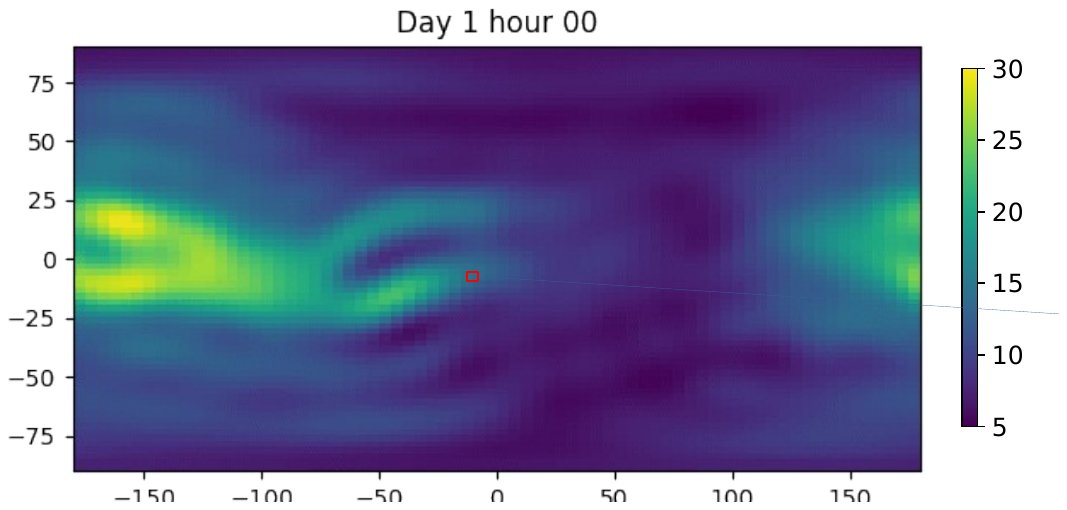
\includegraphics[height=0.3\textheight]{vtec_map}

        {\footnotesize Ionosphere maps (VTEC) of a single day (single band, but colored).}

        \column{0.48\textwidth}
        \centering
        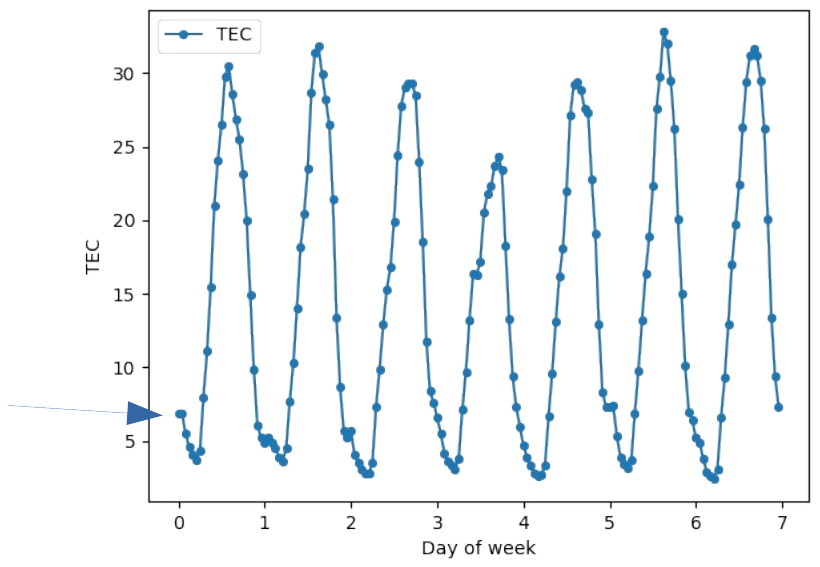
\includegraphics[height=0.3\textheight]{vtec_series}

        {\footnotesize VTEC time series of a single pixel of the map along an entire week.}
    \end{columns}

    \url{https://github.com/mauriciodev/tec_forecast} (Tensorflow 2/Keras)

    \vfill
    {\tiny Paulo MCM de, Marques HA, Feitosa RQ, Ferreira MP (2023) New encoder--decoder convolutional LSTM neural network architectures for next-day global ionosphere maps forecast. GPS Solut 27(2):95. \url{https://doi.org/10.1007/s10291-023-01442-4}}
\end{frame}

\begin{frame}{Prediction of the next maps in a time series}
    \centering
    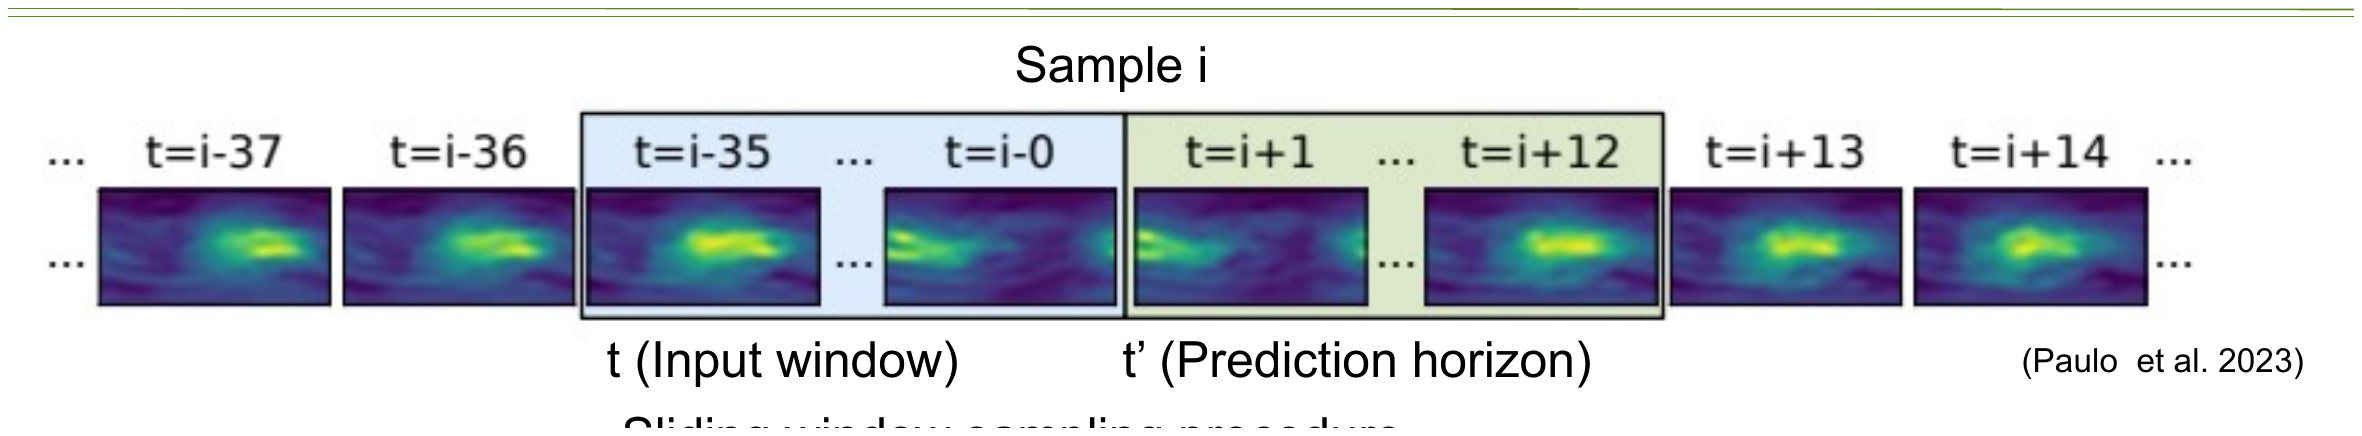
\includegraphics[width=0.9\textwidth]{sliding_window}

    {\footnotesize Sliding window sampling procedure.}

    \begin{columns}[c]
        \column{0.62\textwidth}
        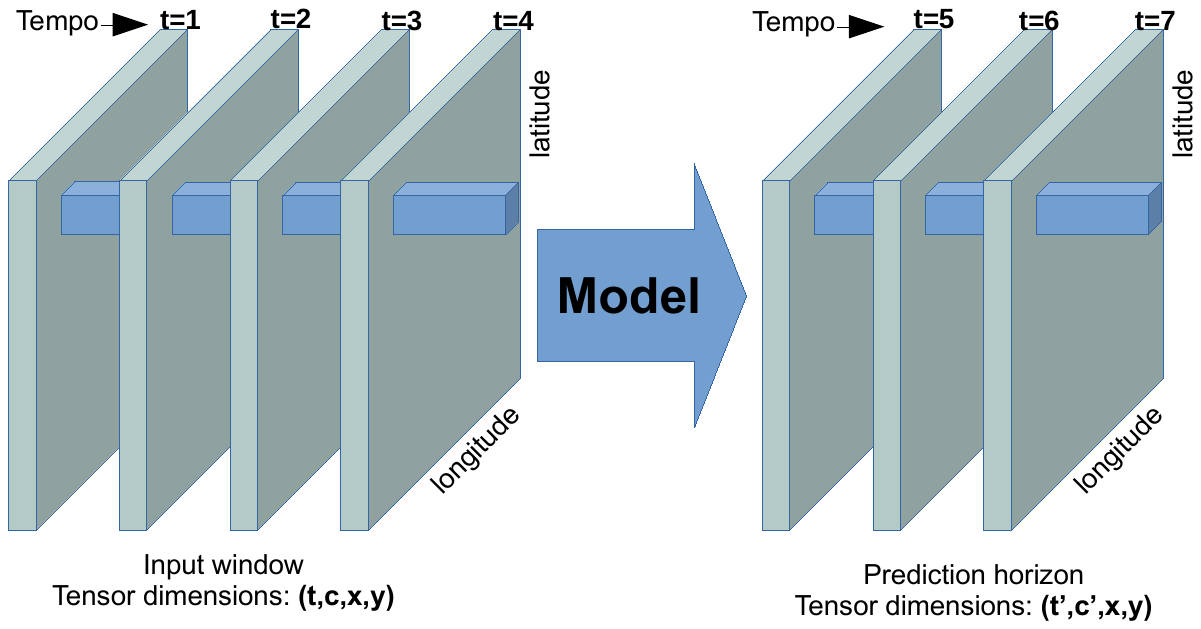
\includegraphics[width=\columnwidth]{model_tensors}

        \column{0.36\textwidth}
        \footnotesize
        Main loss functions:
        \[
        MAE = \frac{\sum_{i=1}^{n} |y_i - \hat{y}_i|}{n}
        \]
        \[
        RMSE = \sqrt{\frac{\sum_{i=1}^{n} (y_i - \hat{y}_i)^2}{n}}
        \]
    \end{columns}

    {\footnotesize The model transforms from $t$ input images to the next $t'$ predicted images.}
\end{frame}

% ============================================================
\section{Data set construction}
% ============================================================

\begin{frame}{Hyperparameters}
    \begin{columns}[t]
        \column{0.45\textwidth}
        \begin{itemize}
            \item Sequences of images
            \begin{itemize}
                \item Time, channels, x, y
            \end{itemize}
            \item PyTorch
            \begin{itemize}
                \item Input: $(t, c, x, y)$
                \item Output: $(t', c', x, y)$
            \end{itemize}
        \end{itemize}

        \espaco
        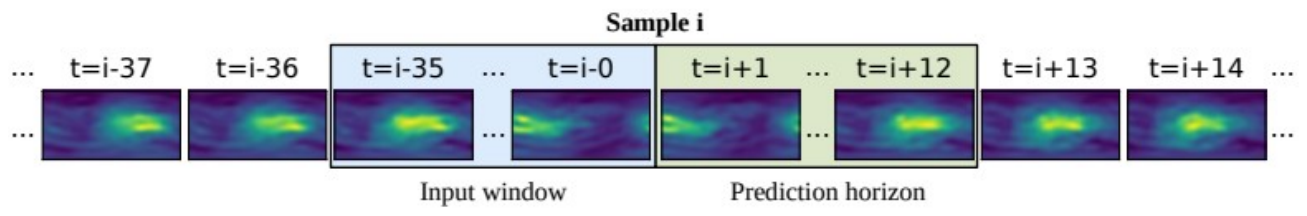
\includegraphics[width=\columnwidth]{sampling_strip}

        {\footnotesize How do we slice it to produce samples? {\tiny (Paulo et al. 2023)}}

        \column{0.52\textwidth}
        \small
        \begin{itemize}
            \item \textbf{Input sequence length ($t$)}
            \begin{itemize}
                \item Must be long enough to provide data for the prediction process.
            \end{itemize}
            \item \textbf{Output sequence length ($t'$)}
            \begin{itemize}
                \item Must be long enough to be usable.
            \end{itemize}
            \item \textbf{Spatial resolution}
            \begin{itemize}
                \item Spatial tensor dimensions $(x,y)$
                \item Multiples of $2^n$, where $n$ is the number of pooling layers.
            \end{itemize}
            \item \textbf{Temporal resolution}
            \begin{itemize}
                \item Must be compatible with the event.
            \end{itemize}
        \end{itemize}
    \end{columns}
\end{frame}

\begin{frame}{Exploring the data}
    \begin{columns}[t]
        \column{0.45\textwidth}
        \small
        \begin{itemize}
            \item Hyperparameters definition
            \begin{itemize}
                \item Previous research
                \item Trial and error
                \item Hyperparameters search (Don't have to be fancy)
            \end{itemize}
            \item Time dimension
            \begin{itemize}
                \item Trend
                \item Season
                \item Noise
            \end{itemize}
            \item Spatial dimensions
            \begin{itemize}
                \item Spatial relations
                \item Clusters, spatial trends, etc
            \end{itemize}
        \end{itemize}

        \column{0.53\textwidth}
        \centering
        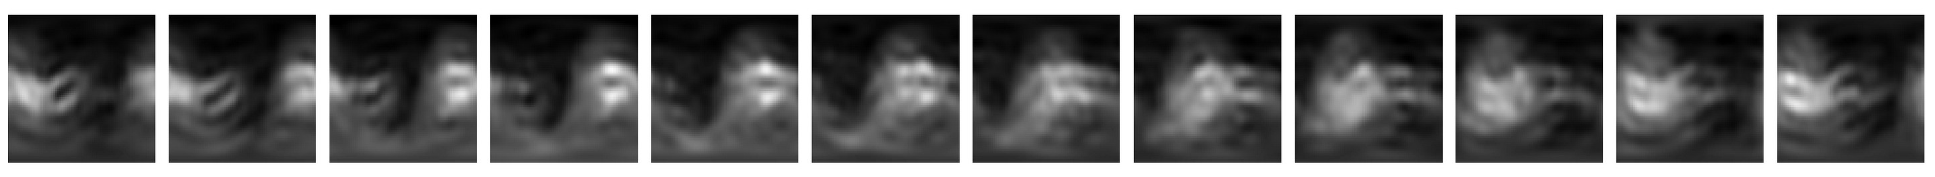
\includegraphics[width=\columnwidth]{image_sequence}

        {\footnotesize Image sequence.}

        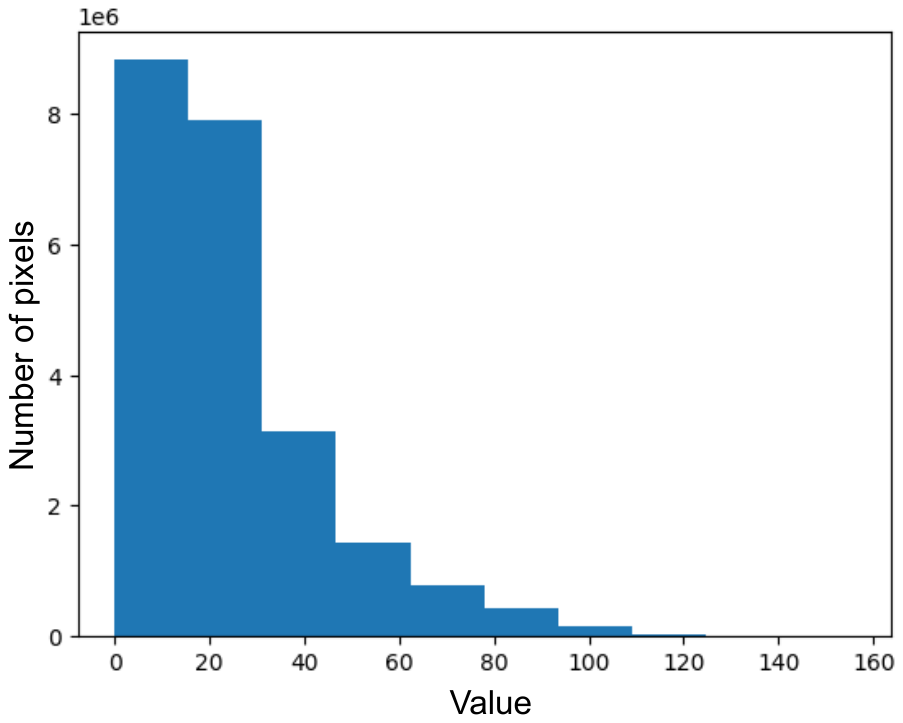
\includegraphics[height=0.4\textheight]{histogram}

        {\footnotesize Flattened data histogram.\\ $(t,c,x,y) \rightarrow (t \cdot x \cdot y, c)$}
    \end{columns}
\end{frame}

\begin{frame}{Exploring the data}
    \begin{columns}[t]
        \column{0.45\textwidth}
        \centering
        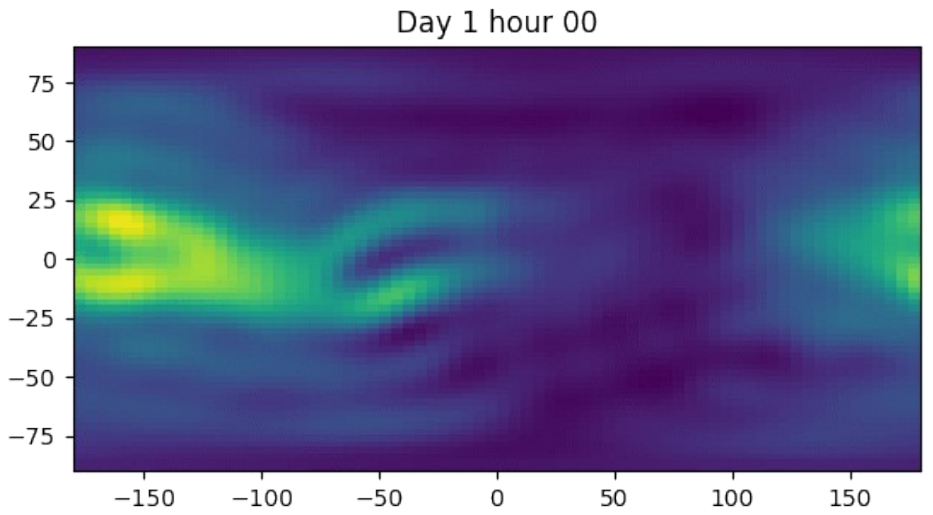
\includegraphics[width=\columnwidth]{map_day1}

        {\footnotesize Video sequences can help understand the spatiotemporal trends.}

        \column{0.53\textwidth}
        \centering
        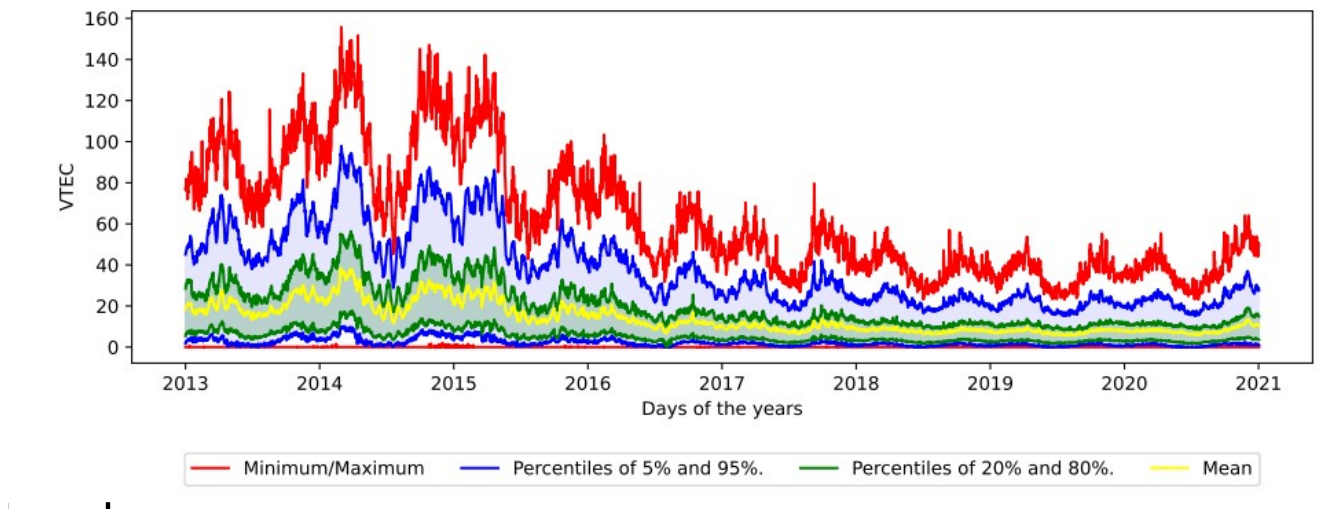
\includegraphics[width=\columnwidth]{percentiles}

        {\footnotesize Percentiles of the reshaped tensor.\\ $(t,c,x,y) \rightarrow (t, c \cdot x \cdot y)$}
    \end{columns}
\end{frame}

% ============================================================
\section{Architectures}
% ============================================================

\begin{frame}{Architectures}
    \begin{itemize}
        \item Recurrent neural networks
        \item 3D Convolutional networks
        \item 2D Convolutional networks (based on SimVP)
        \item Transformers networks
        \item Structured state space sequence models (SSM)
    \end{itemize}
\end{frame}

\begin{frame}{Recurrent neural networks: ConvLSTM}
    \begin{columns}[c]
        \column{0.36\textwidth}
        \footnotesize
        $H_i = f(X_i, H_{i-1}, C_{i-1})$\\
        With: $H_0 = 0$ e $C_0 = 0$

        \espaco
        $X_i$: input data of current frame;\\
        $H_i$: output of current frame;\\
        $H_{i-1}$: output of the previous frame;\\
        $C_{i-1}$: memory cell of the previous frame.

        \column{0.62\textwidth}
        \centering
        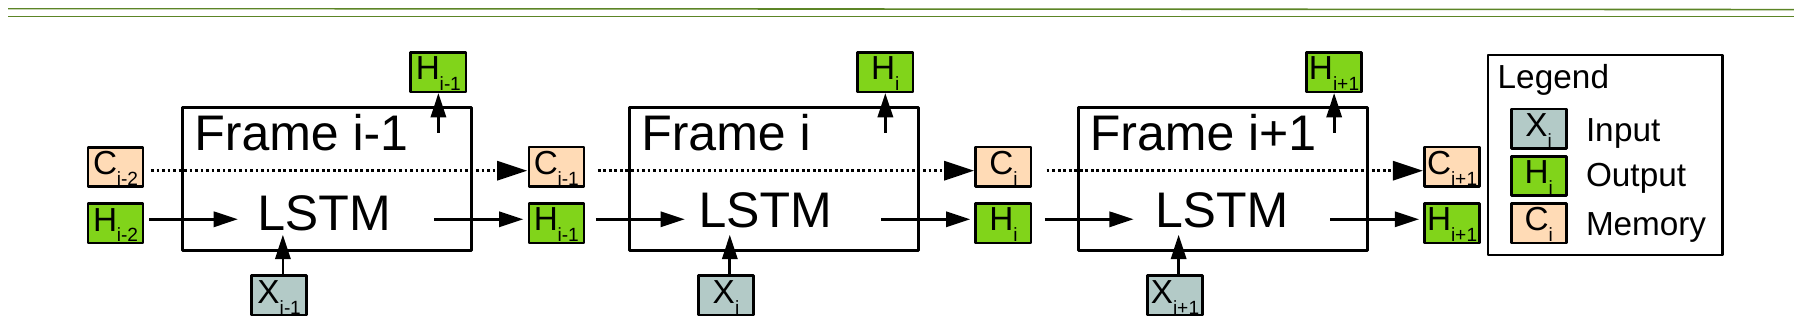
\includegraphics[width=\columnwidth]{convlstm_cell}

        {\tiny Recurrent LSTM cell processing for frames $X_{i-1}$, $X_i$ e $X_{i+1}$}
    \end{columns}

    \espaco
    \begin{columns}[b]
        \column{0.27\textwidth}
        \centering
        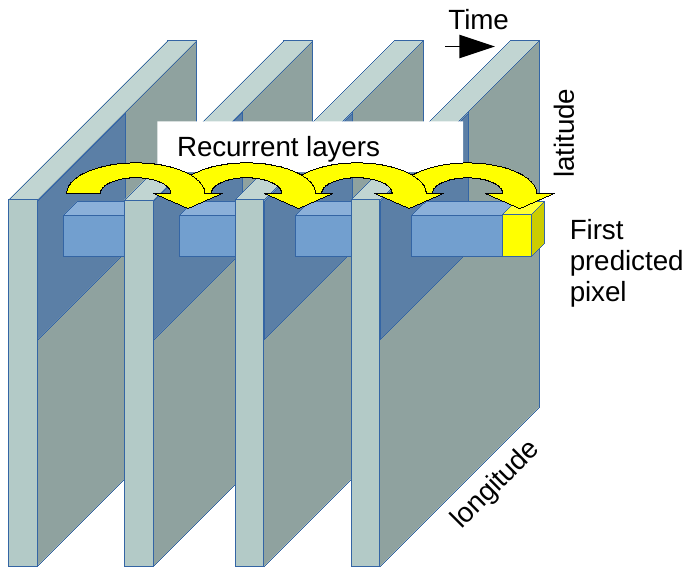
\includegraphics[width=\columnwidth]{rnn_stack}

        {\tiny Single step prediction with RNN}

        \column{0.71\textwidth}
        \centering
        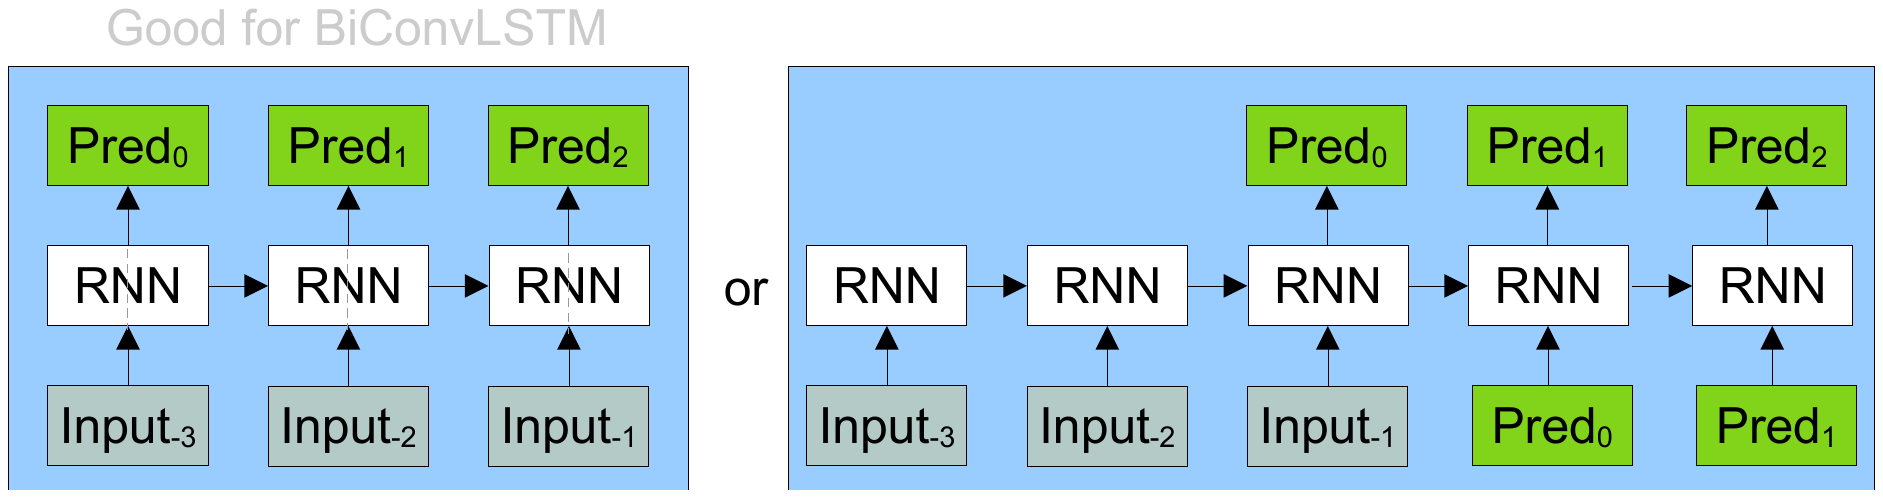
\includegraphics[width=\columnwidth]{rnn_methods}

        {\footnotesize Prediction methods with one RNN}
    \end{columns}
\end{frame}

\begin{frame}{Recurrent neural networks: ED-ConvLSTM}
    \begin{columns}[c]
        \column{0.48\textwidth}
        \centering
        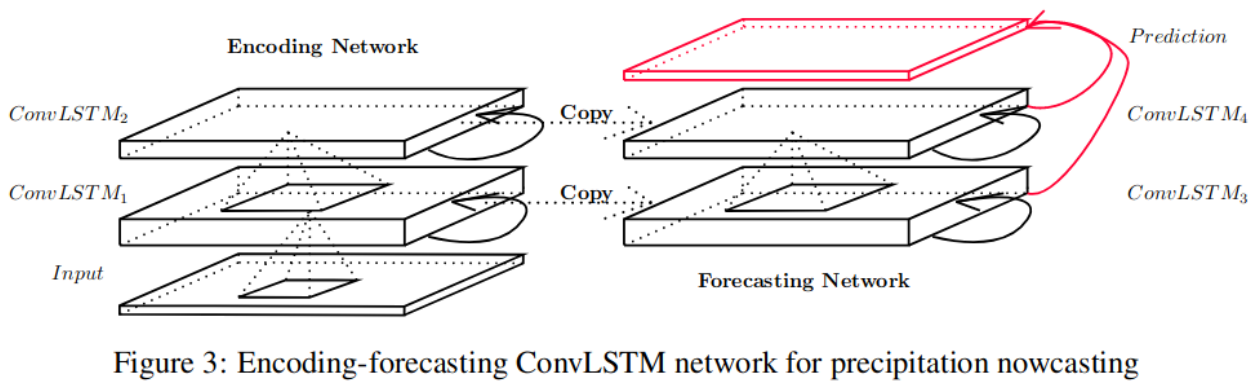
\includegraphics[width=\columnwidth]{shi_convlstm}

        {\footnotesize ConvLSTM was actually first designed with different layers for encoding and forecasting. (Shi et al. 2015)}

        \column{0.48\textwidth}
        \centering
        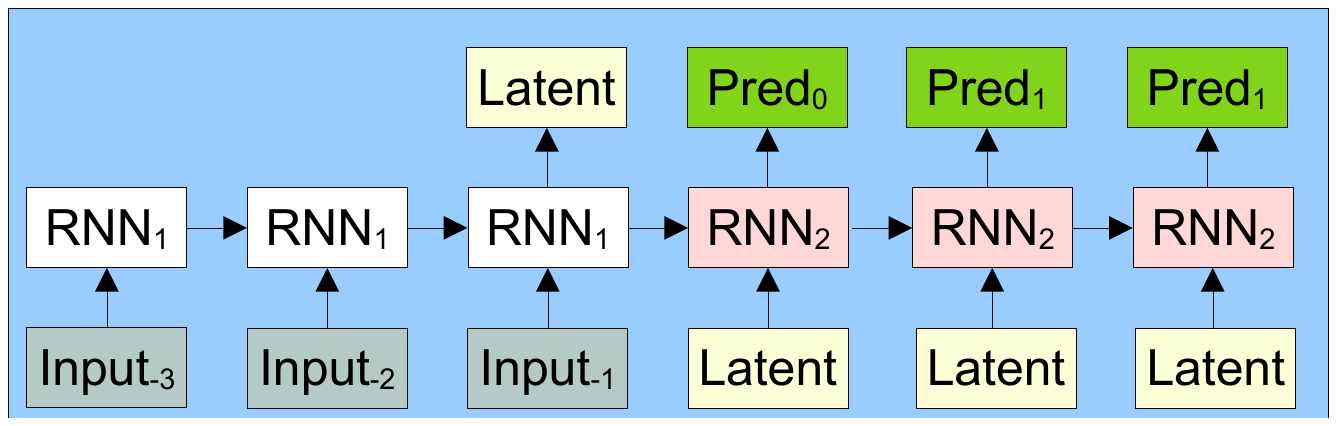
\includegraphics[width=\columnwidth]{ed_convlstm}

        {\footnotesize Prediction method with Encoder-Decoder ConvLSTM.}
    \end{columns}

    \vfill
    \begin{center}
        Most articles ignore the difference between ConvLSTM and ED-ConvLSTM, but there are articles that show the error propagation.
    \end{center}
\end{frame}

\begin{frame}{Recurrent Neural Networks evolution}
    \begin{itemize}
        \item ConvLSTM (2015)
        \begin{itemize}
            \item Uses a Memory Cell ($C$) that stores information through time steps.
            \item 2D convolutions on each frame.
        \end{itemize}
        \item PredRNN (2017) {\tiny extends ConvLSTM}
        \begin{itemize}
            \item ST-LSTM: Adds a new memory tensor ($M$) that is passed through stacked RNN layers.
        \end{itemize}
        \item E3D-LSTM (2018) {\tiny extends PredRNN}
        \begin{itemize}
            \item 3D Convolutions instead of 2D.
            \item Attention mechanism on tensor $C$.
        \end{itemize}
        \item PredRNN v2 (2022) {\tiny extends PredRNN}
        \begin{itemize}
            \item Adds a decoupled loss to learn different features with $C$ and $M$.
        \end{itemize}
        \item \textbf{Future?: XLSTM (2024) there is no ConvXLSTM yet.}
    \end{itemize}

    \vfill
    {\footnotesize References can be found in OpenSTL GitHub page.}
\end{frame}

\begin{frame}{Remembering convolutional layers}
    \centering
    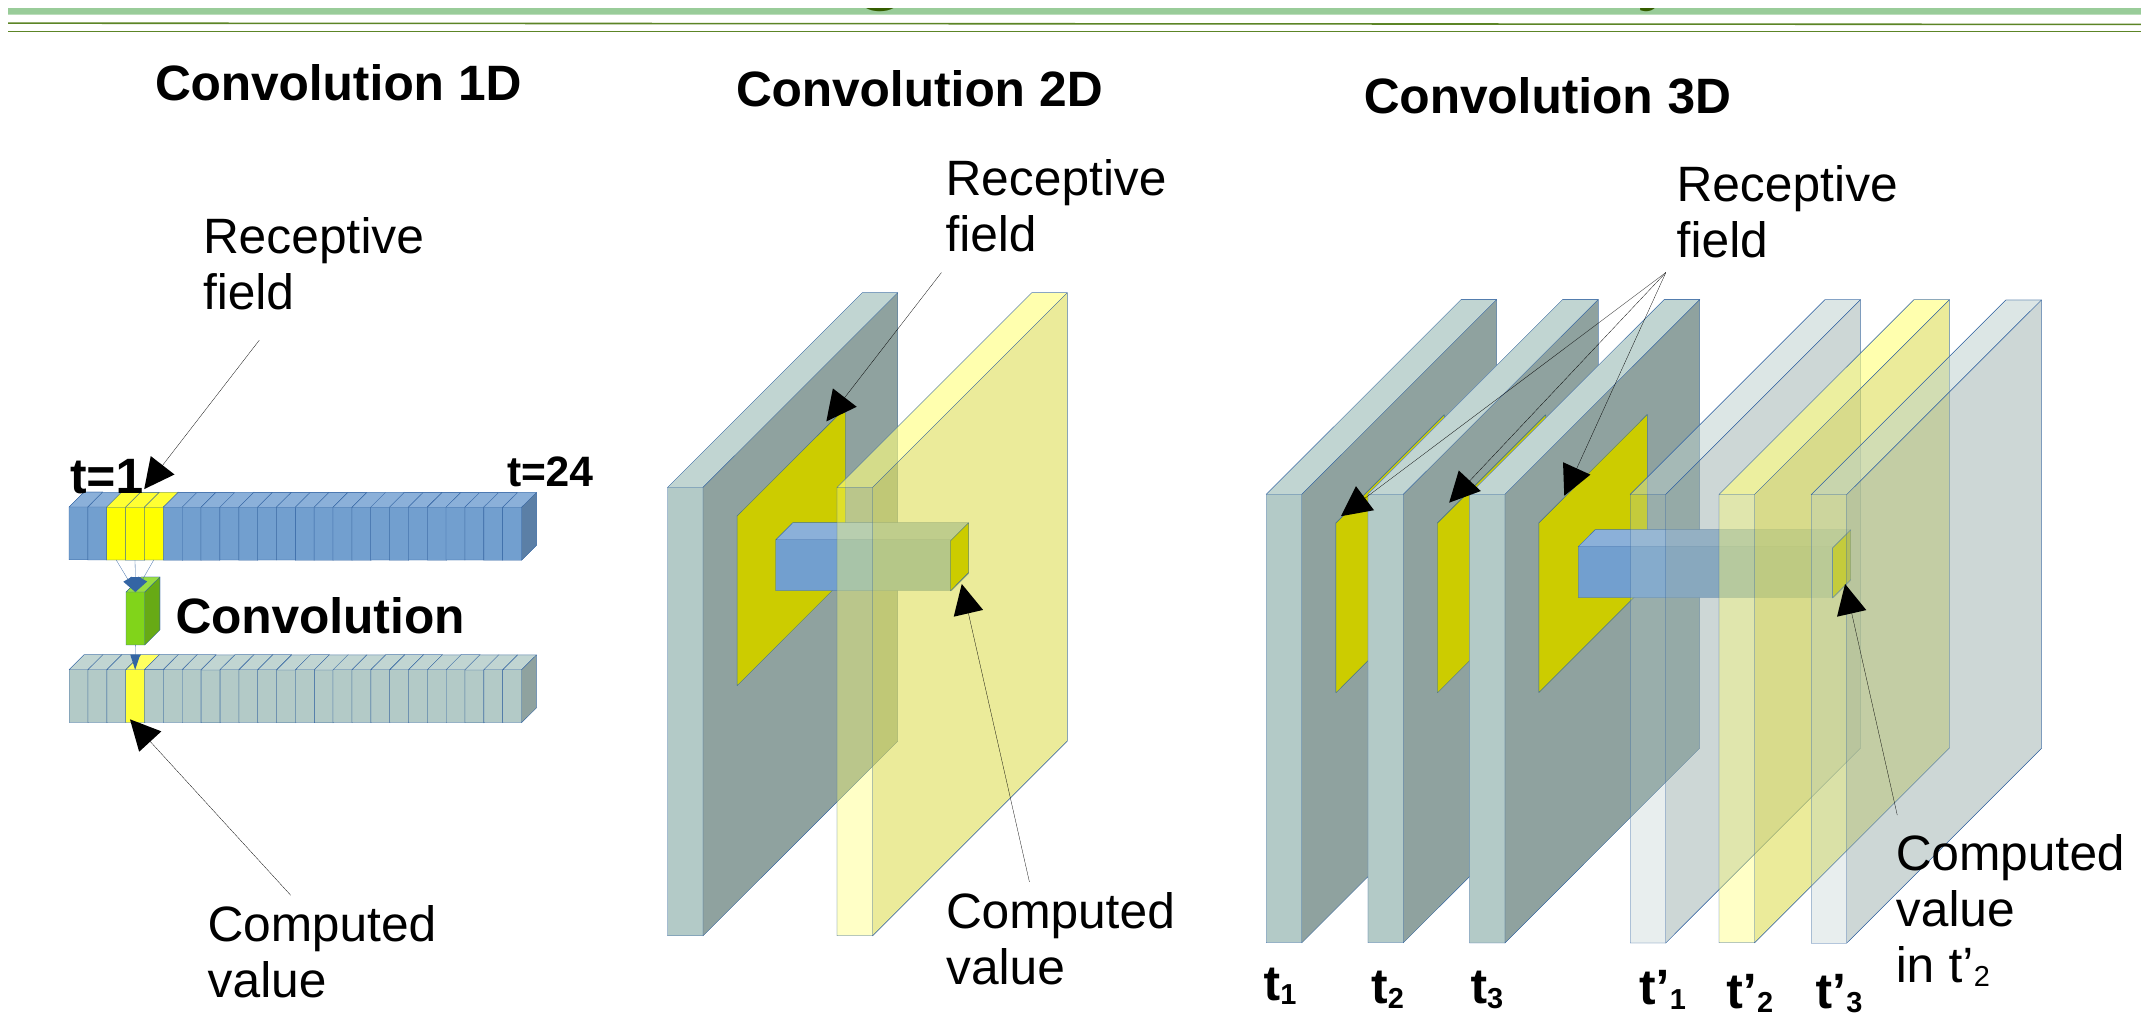
\includegraphics[height=0.72\textheight]{convolutions}

    {\footnotesize Obs.: 3D convolutions with stride 1 and pad do not modify the $t,x,y$ dimensions.}
\end{frame}

\begin{frame}{3D Convolutional networks: Broad-UNet (3D)}
    \begin{itemize}
        \item Broad-UNet: Multi-scale feature learning for nowcasting tasks
        \item \url{https://github.com/jesusgf96/Broad-UNet}
    \end{itemize}
    \begin{columns}[c]
        \column{0.62\textwidth}
        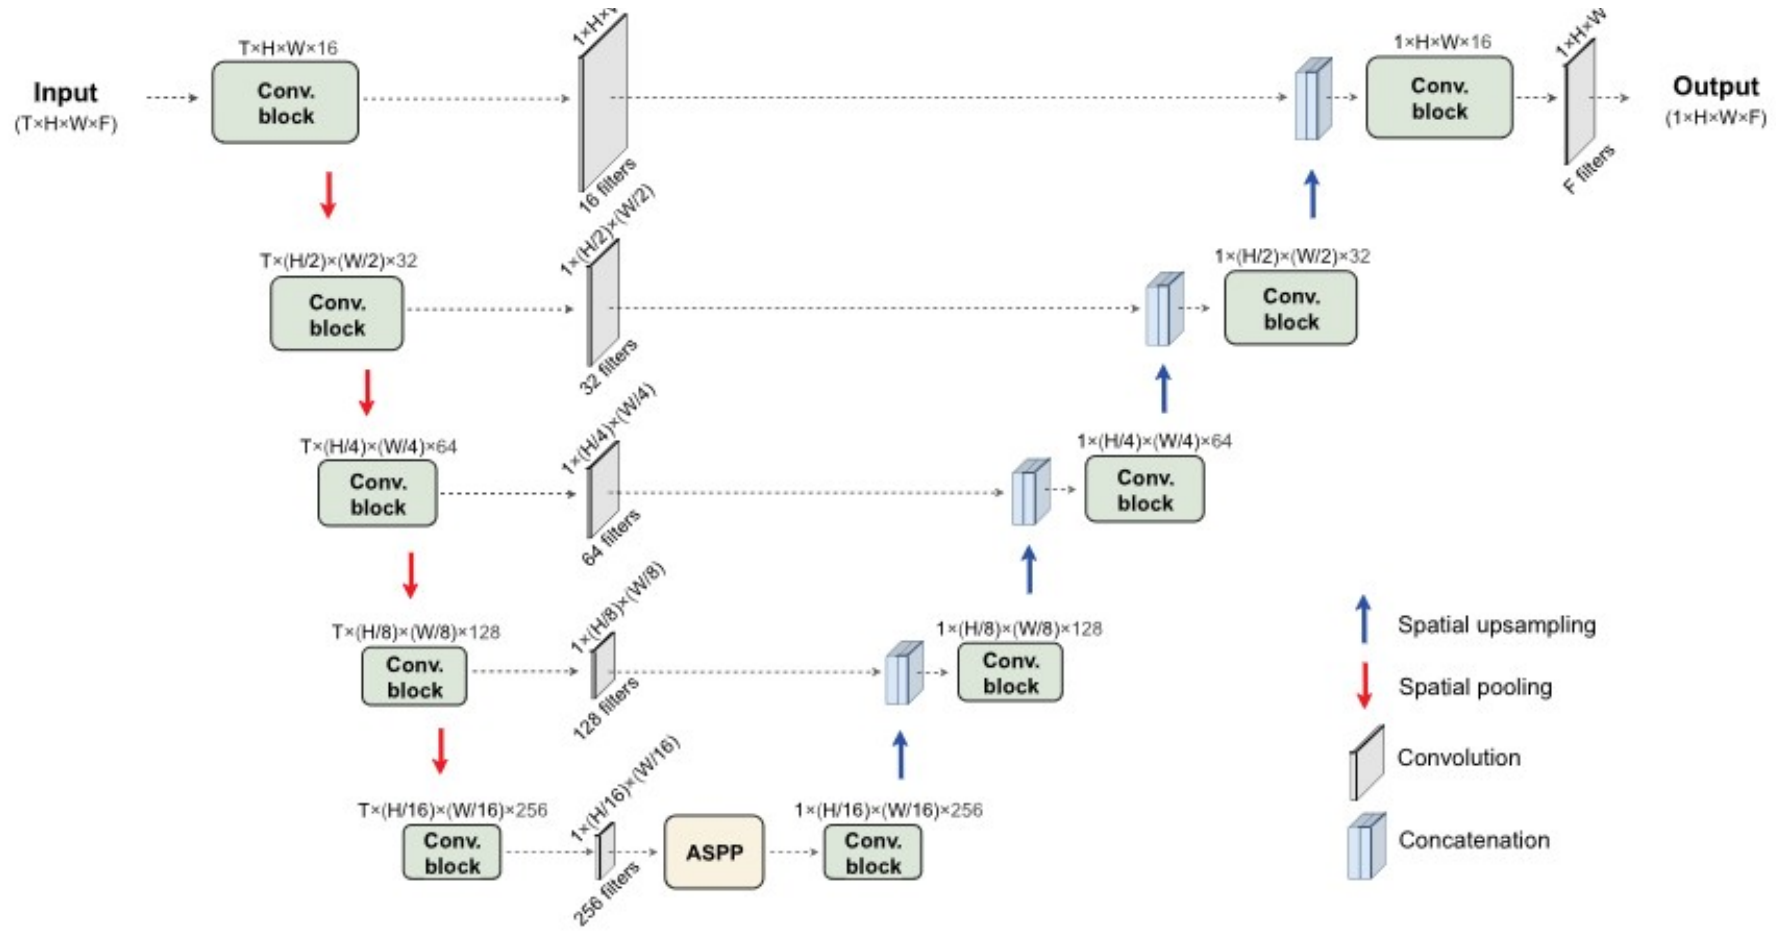
\includegraphics[width=\columnwidth]{broad_unet}

        \column{0.36\textwidth}
        \centering
        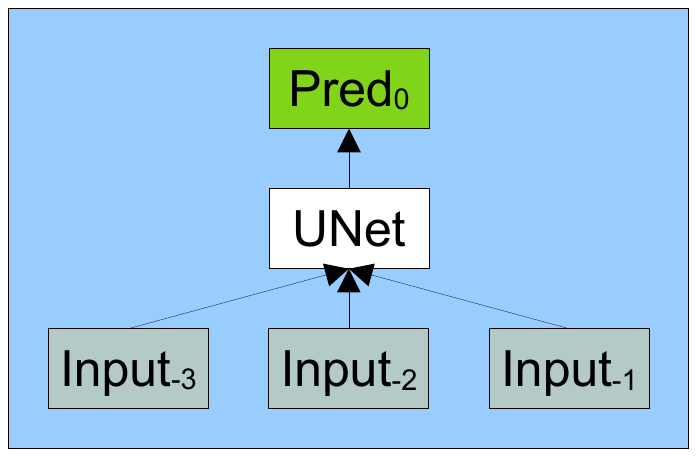
\includegraphics[width=0.6\columnwidth]{broad_unet_pred}

        {\footnotesize Prediction method with Broad-Unet 3D}

        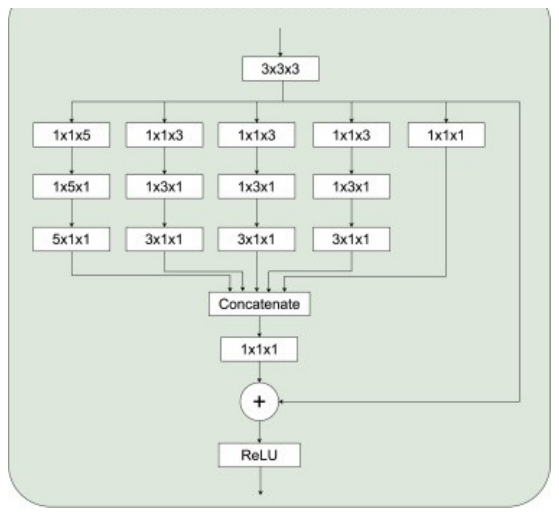
\includegraphics[height=0.3\textheight]{multiscale_block}
    \end{columns}

    \hfill{\tiny (Fernández and Mehrkanoon 2021)}
\end{frame}

\begin{frame}{3D Convolutional networks: UNet 3D}
    \begin{columns}[c]
        \column{0.6\textwidth}
        \centering
        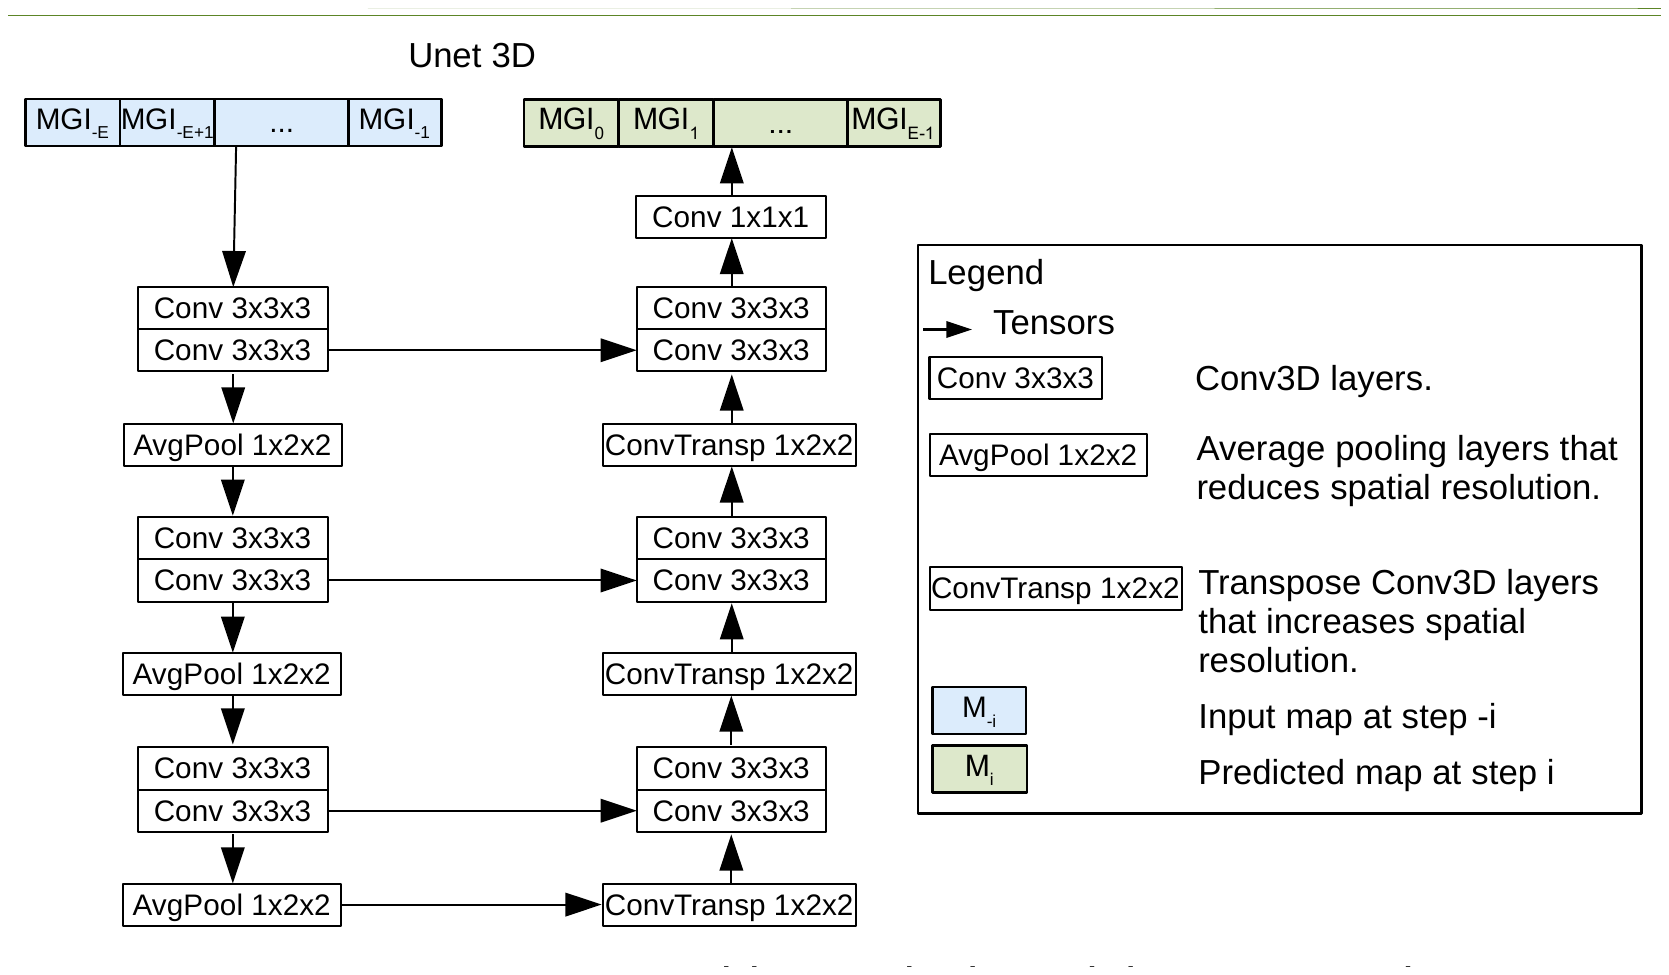
\includegraphics[width=\columnwidth]{unet3d}

        {\footnotesize \textbf{UNet3D} architecture: hierarquical spatial representation widens the spatial receptive field of each predicted pixel.}

        \column{0.38\textwidth}
        \centering
        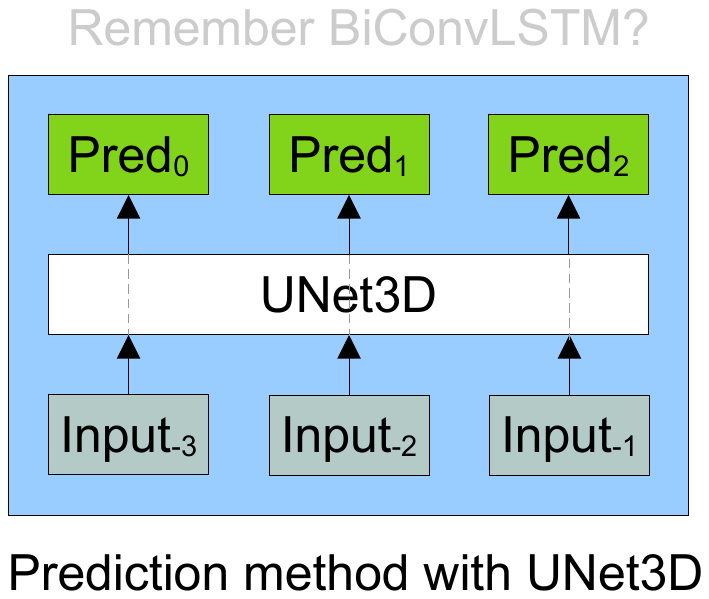
\includegraphics[width=\columnwidth]{unet3d_pred}
    \end{columns}
\end{frame}

\begin{frame}{2D Convolutional networks: SimVP v2}
    \begin{columns}[c]
        \column{0.58\textwidth}
        \centering
        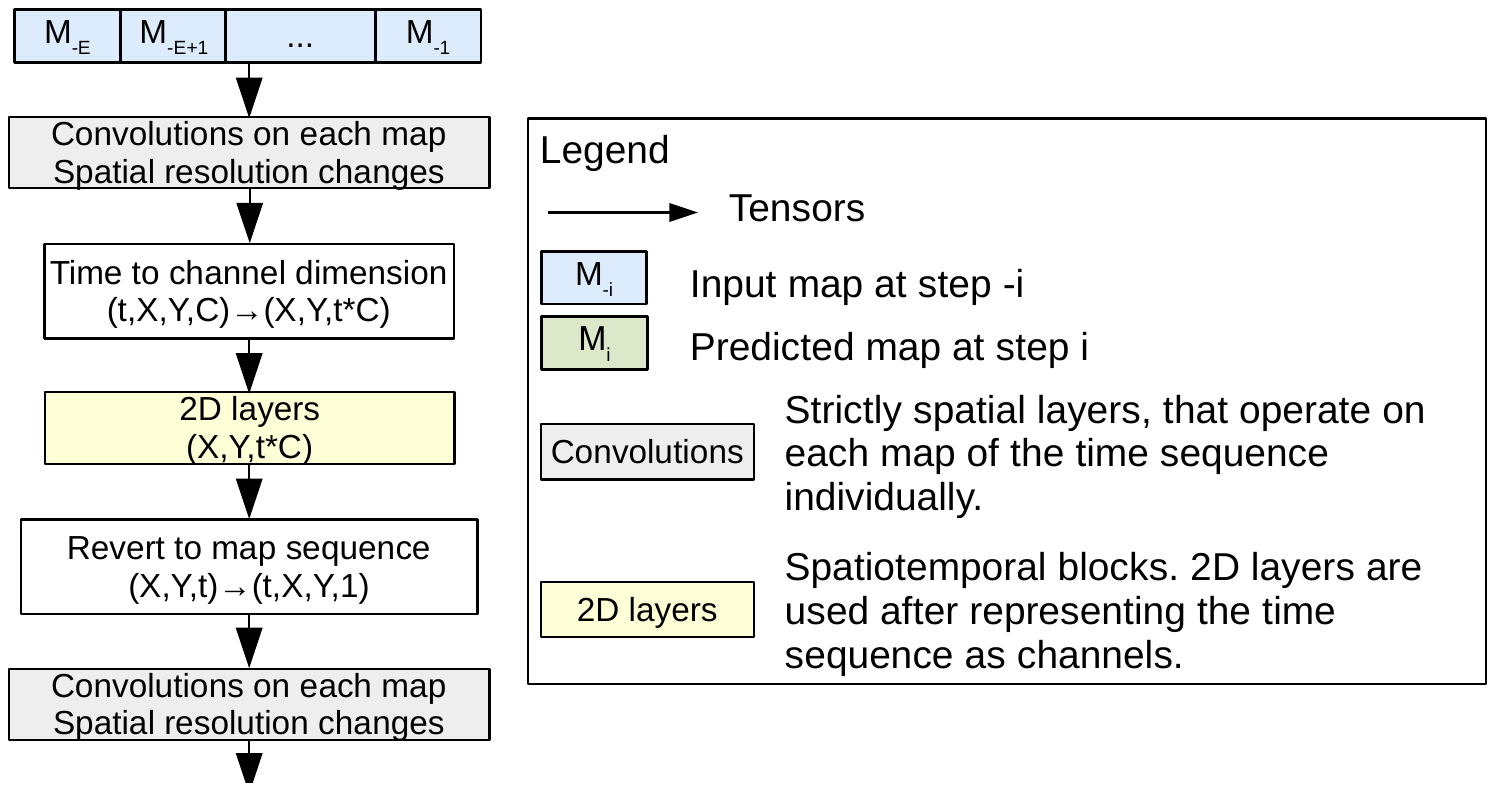
\includegraphics[width=\columnwidth]{simvp}

        {\footnotesize \textbf{SimVP} architecture (TAN et al., 2022): The time dimension is represented in the channel dimension, thus 2D layers can be used to processes sequences of maps.}

        \column{0.4\textwidth}
        \centering
        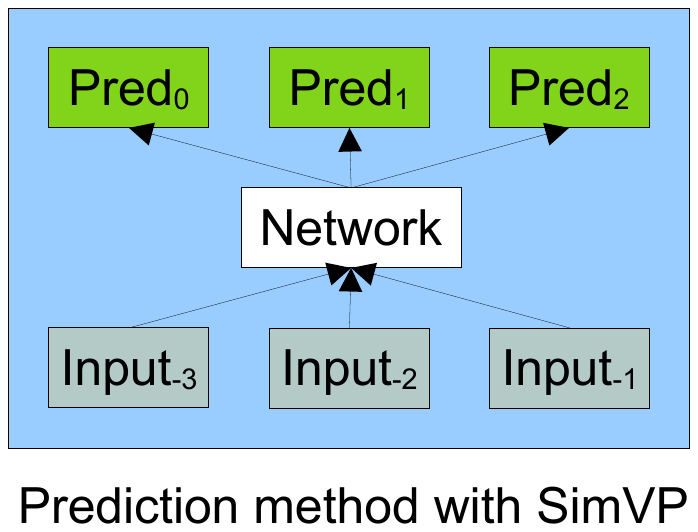
\includegraphics[width=0.9\columnwidth]{simvp_pred}

        \espaco
        \small
        The receptive field in the time dimension is the entire time sequence for each pixel.

        \espaco
        Downside: Too many values on each neuron.
    \end{columns}
\end{frame}

\begin{frame}{2D Convolutional networks: SimVP v2}
    \begin{columns}[c]
        \column{0.48\textwidth}
        \centering
        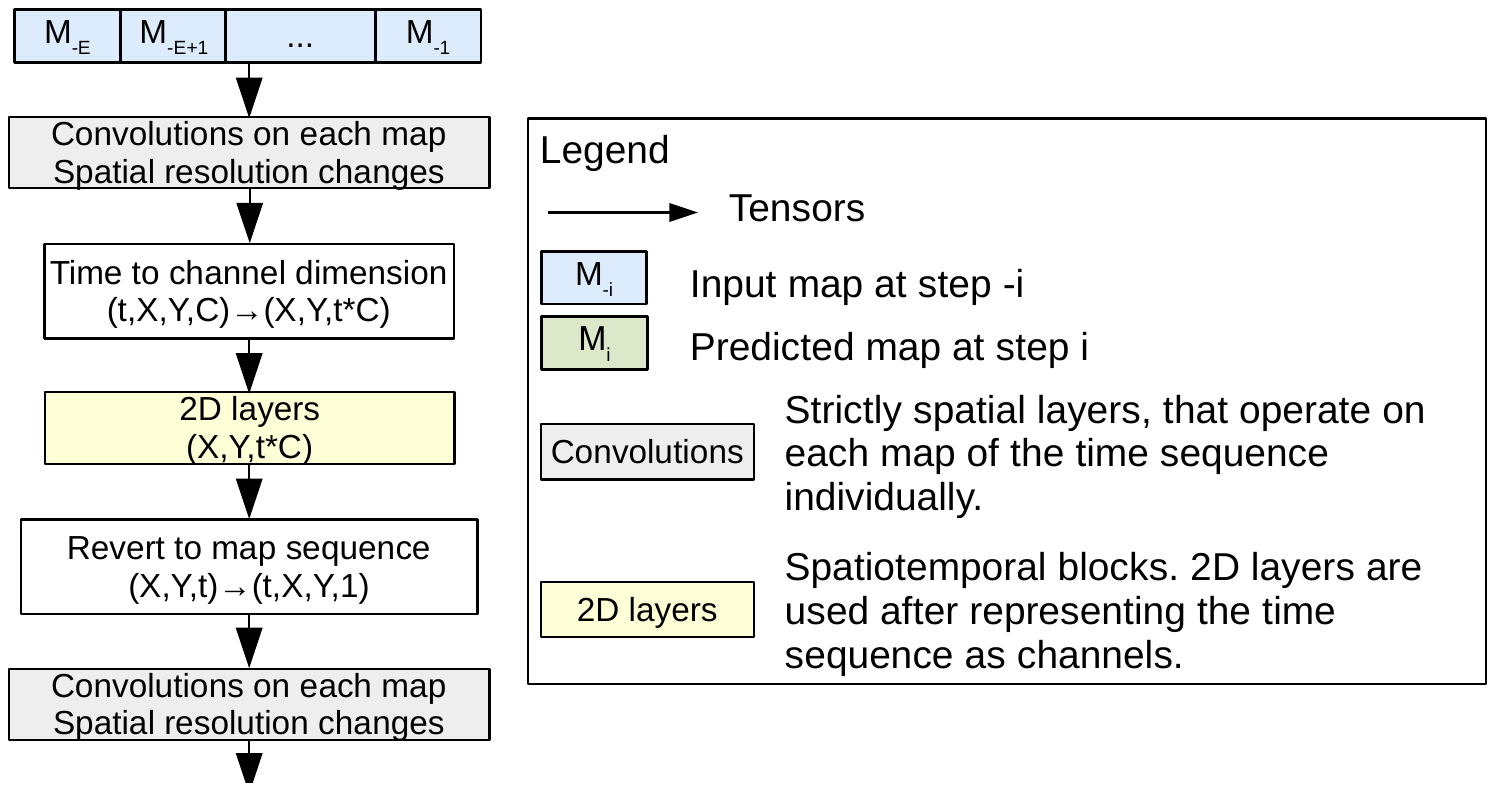
\includegraphics[width=\columnwidth]{simvp}

        {\tiny \textbf{SimVP} architecture (TAN et al., 2022): The time dimension is represented in the channel dimension, thus 2D layers can be used to processes sequences of maps.}

        \column{0.5\textwidth}
        \centering
        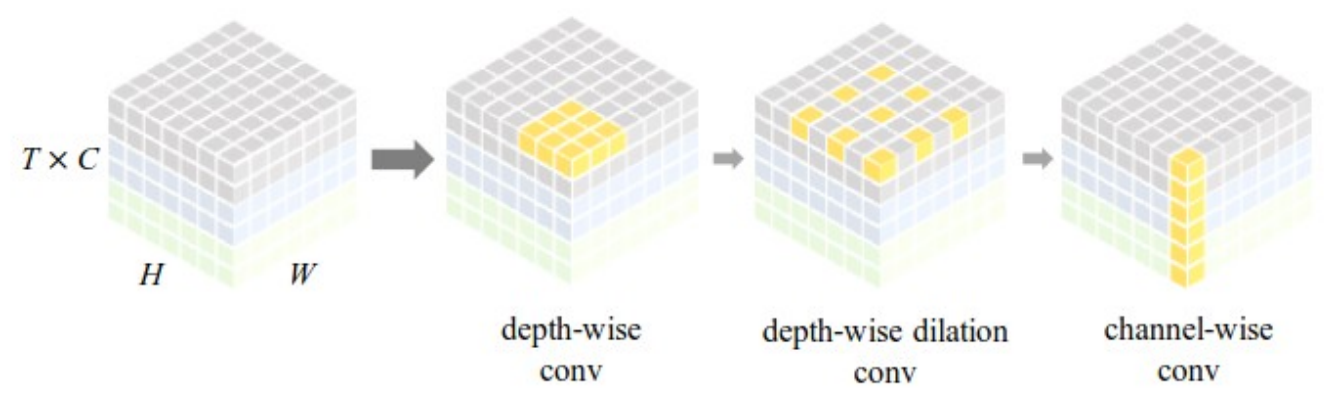
\includegraphics[width=0.9\columnwidth]{gsta}

        {\tiny Fig. 7. The large kernel convolution in the gated spatiotemporal attention module. The yellow region denotes the receptive field.}

        {\footnotesize Gated Spatiotemporal Attention Translator (gSTA)\\
        \url{https://github.com/chengtan9907/OpenSTL}}

        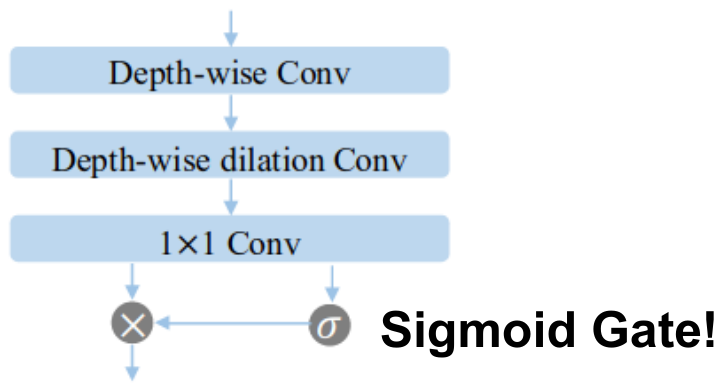
\includegraphics[height=0.2\textheight]{gsta_gate}

        \hfill{\tiny (Tan et al. 2022)}
    \end{columns}
\end{frame}

\begin{frame}{Remembering Transformer concepts}
    \begin{columns}[c]
        \column{0.48\textwidth}
        \footnotesize
        Natural Language processing

        Memory: $O(\text{tokens}^2)$

        \centering
        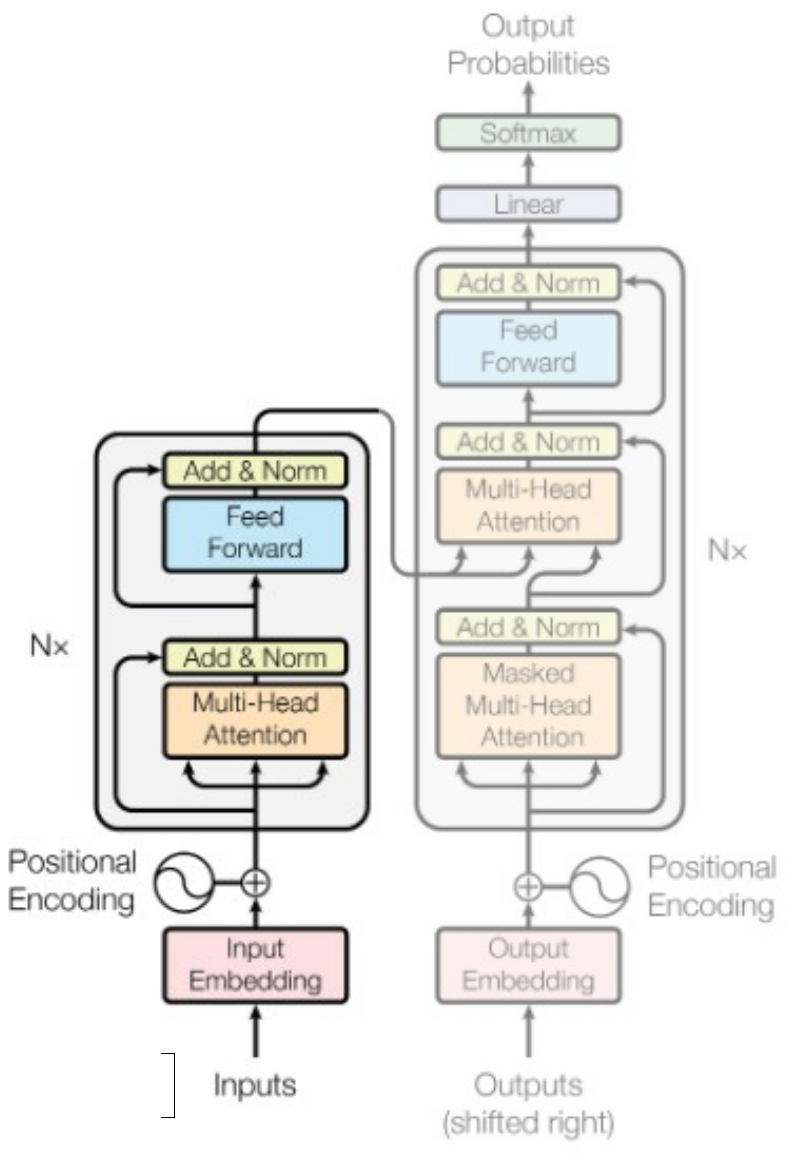
\includegraphics[height=0.55\textheight]{transformer}

        Dimensions: (tokens, channels)

        Transformers architecture {\tiny (Vaswani et al. 2017)}

        \column{0.5\textwidth}
        \centering
        \[
        \text{Attention}(Q,K,V) = \text{softmax}\left(\frac{QK^T}{\sqrt{d_k}}\right)V
        \]

        \begin{columns}[c]
            \column{0.45\columnwidth}
            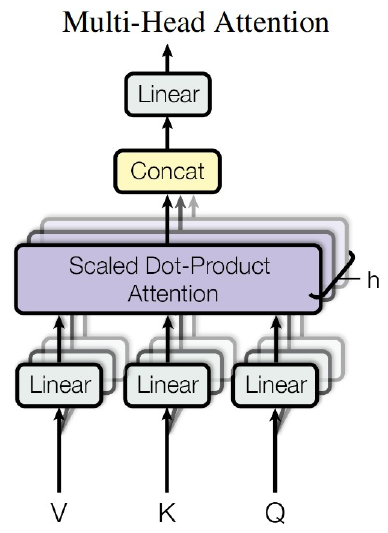
\includegraphics[width=\columnwidth]{multihead}
            \column{0.5\columnwidth}
            \footnotesize Self attention: $Q=V=K$
        \end{columns}

        \espaco
        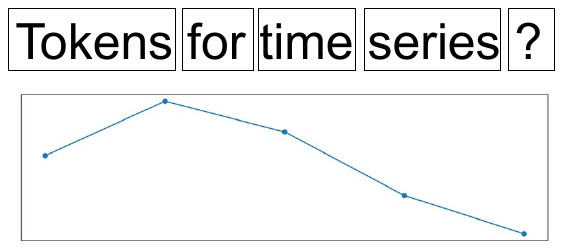
\includegraphics[width=0.5\columnwidth]{tokens_ts}

        {\footnotesize NLP tokens and an 1-D time series.}
    \end{columns}
\end{frame}

\begin{frame}{Transformers for images: ViT and Swin}
    \centering
    From tokens describing words to tokens describing parts of an image.

    These can be used with SimVP for spatiotemporal prediction!

    \espaco
    \begin{columns}[t]
        \column{0.48\textwidth}
        \centering
        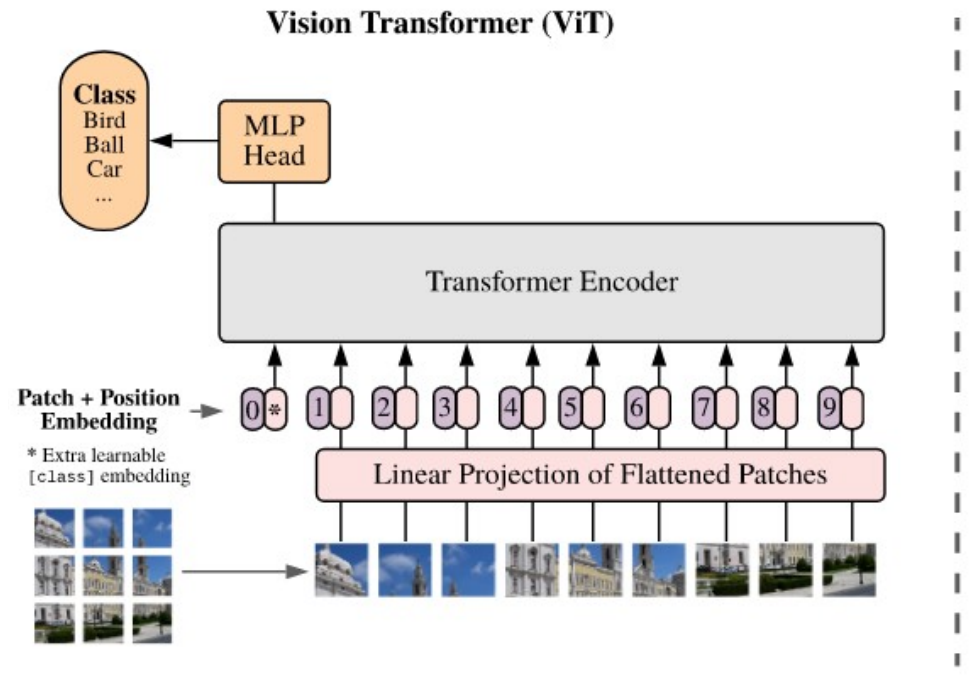
\includegraphics[height=0.45\textheight]{vit}

        {\footnotesize Vision Transformer (ViT): Attention is used to classify the entire image (DOSOVITSKIY et al. 2021)}

        \column{0.48\textwidth}
        \centering
        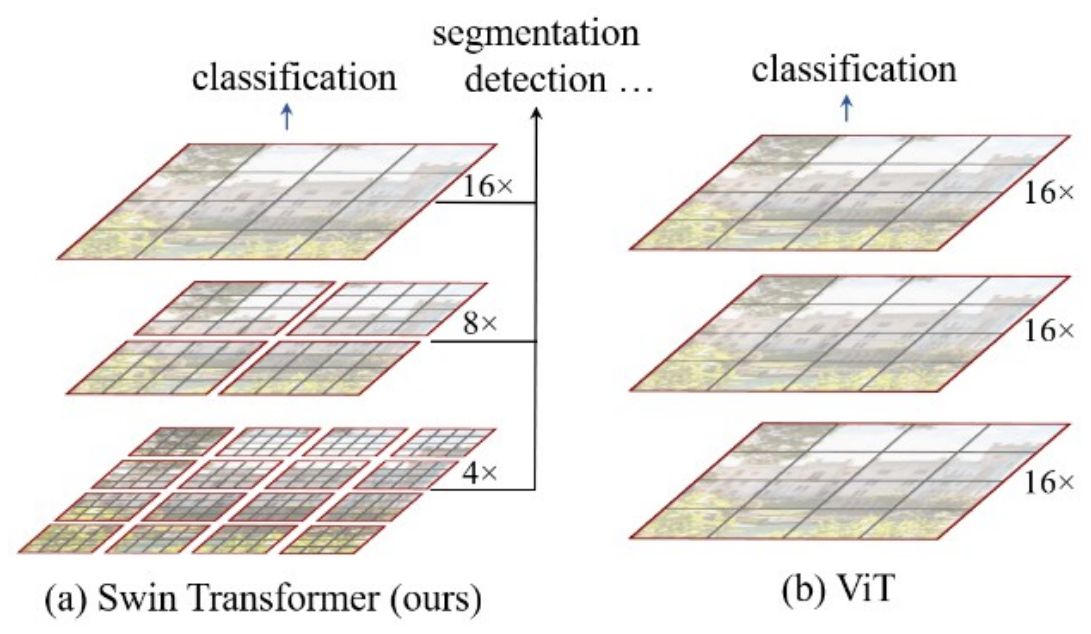
\includegraphics[height=0.45\textheight]{swin}

        {\footnotesize Swin Transformer: Attention is used to describe the neighborhood (LIU et al. 2021)}
    \end{columns}
\end{frame}

\begin{frame}{Transformers for video: ViVit}
    \begin{columns}[c]
        \column{0.5\textwidth}
        \centering
        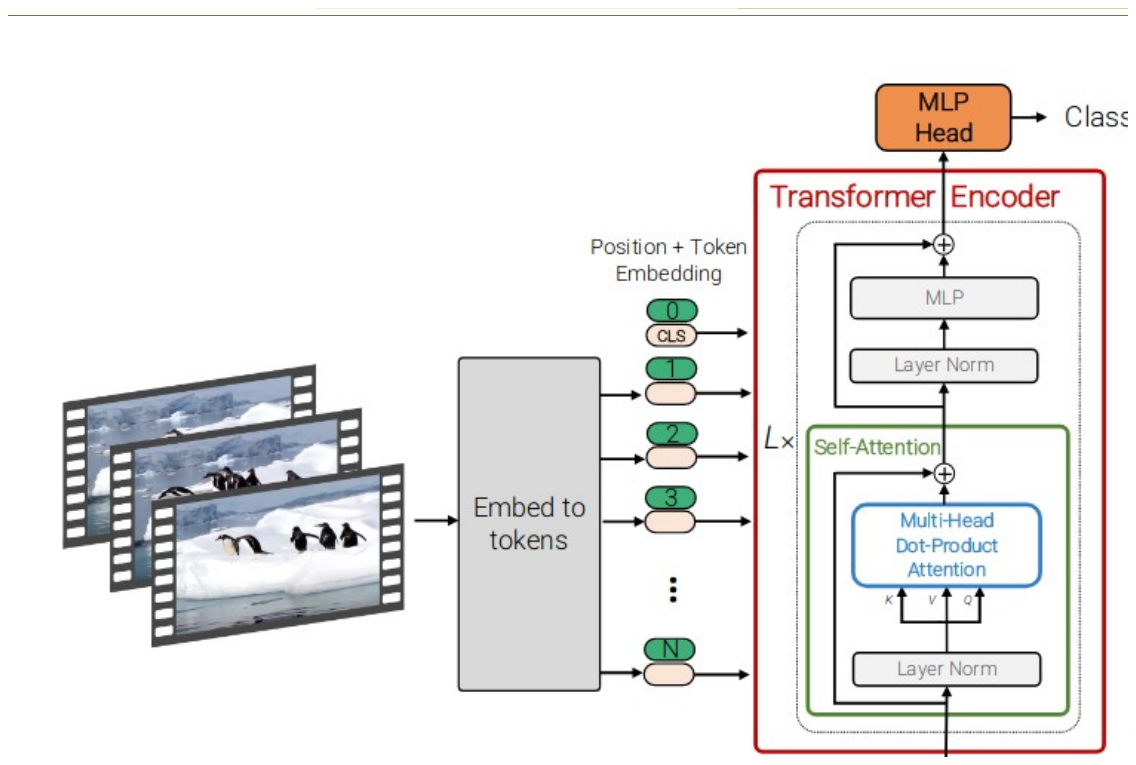
\includegraphics[width=\columnwidth]{vivit}

        {\footnotesize Video Vision Transformer {\tiny (ARNAB et al., 2021)}}

        \espaco
        Similar to Vision Transformer (ViT), ViVit was designed to classify an entire video.

        \column{0.48\textwidth}
        \centering
        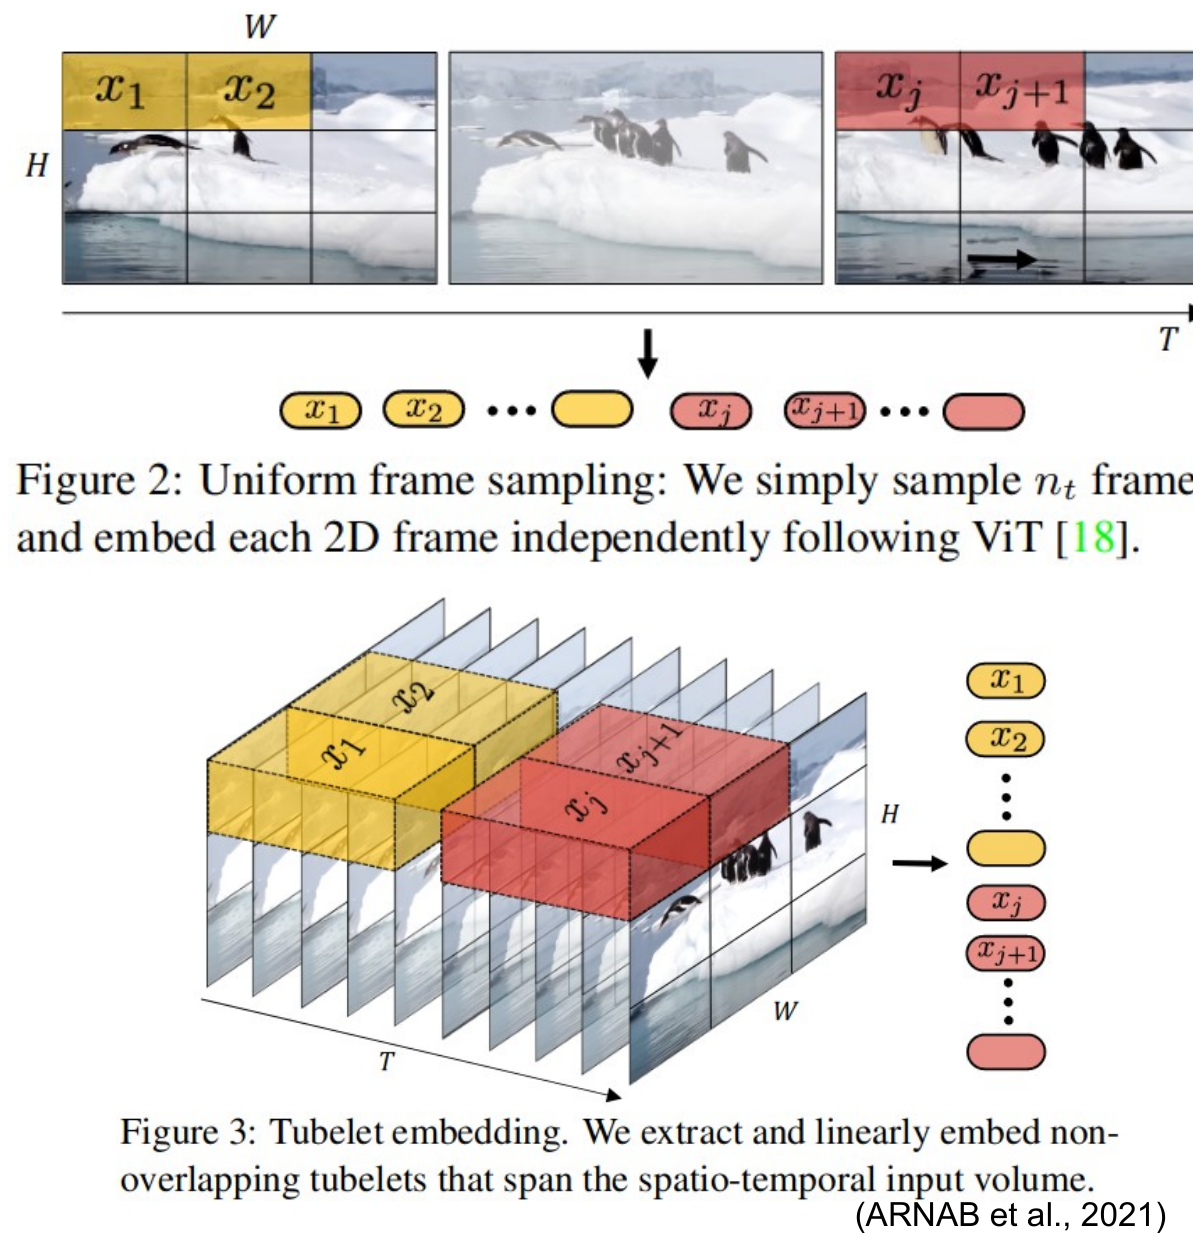
\includegraphics[width=\columnwidth]{vivit_tubelets}
    \end{columns}
\end{frame}

\begin{frame}{Transformers for spatiotemporal prediction}
    \begin{columns}[t]
        \column{0.48\textwidth}
        \begin{itemize}
            \item Earthformer
            \begin{itemize}
                \item Tokens: Cuboid attention
                \item Global features
            \end{itemize}
        \end{itemize}
        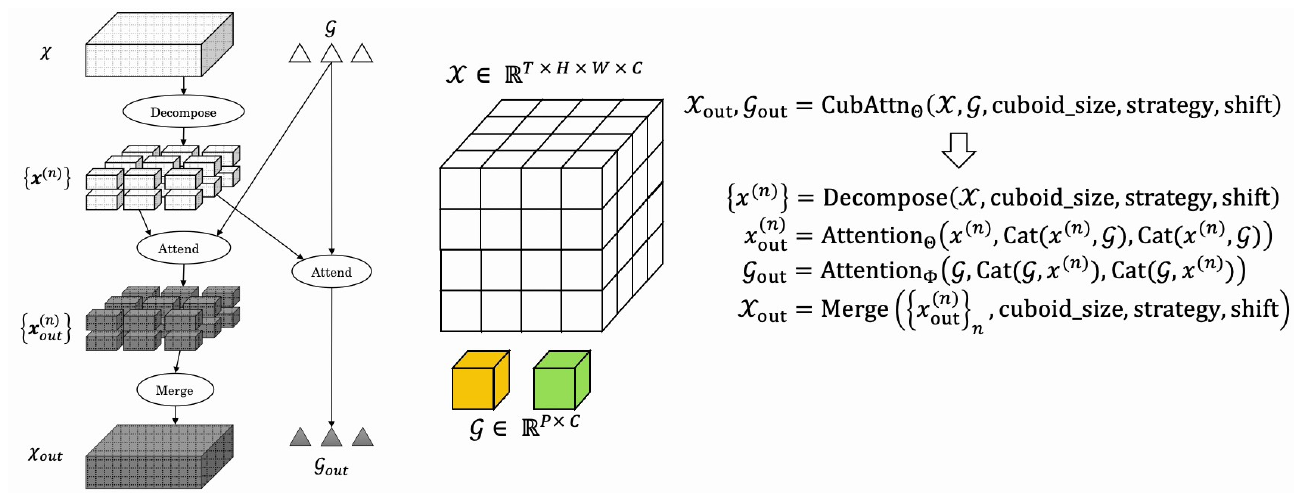
\includegraphics[width=\columnwidth]{earthformer}

        \column{0.48\textwidth}
        \begin{itemize}
            \item MagVIT (MAsked Generative VIdeo Transformer)
            \begin{itemize}
                \item Tokens: 3D-Vector-Quantized (VQ) auto-encoder
                \item Masked token modeling
                \item Multi-task learning
            \end{itemize}
        \end{itemize}
    \end{columns}

    \vfill
    {\scriptsize
    Earthformer (PyTorch): \url{https://github.com/amazon-science/earth-forecasting-transformer} (Gao et al. 2022)\\
    MagVIT (Google Jax): \url{https://github.com/google-research/magvit} (Yu et al. 2023)}
\end{frame}

\begin{frame}{Recurrent neural network (again?): SwinLSTM}
    \centering
    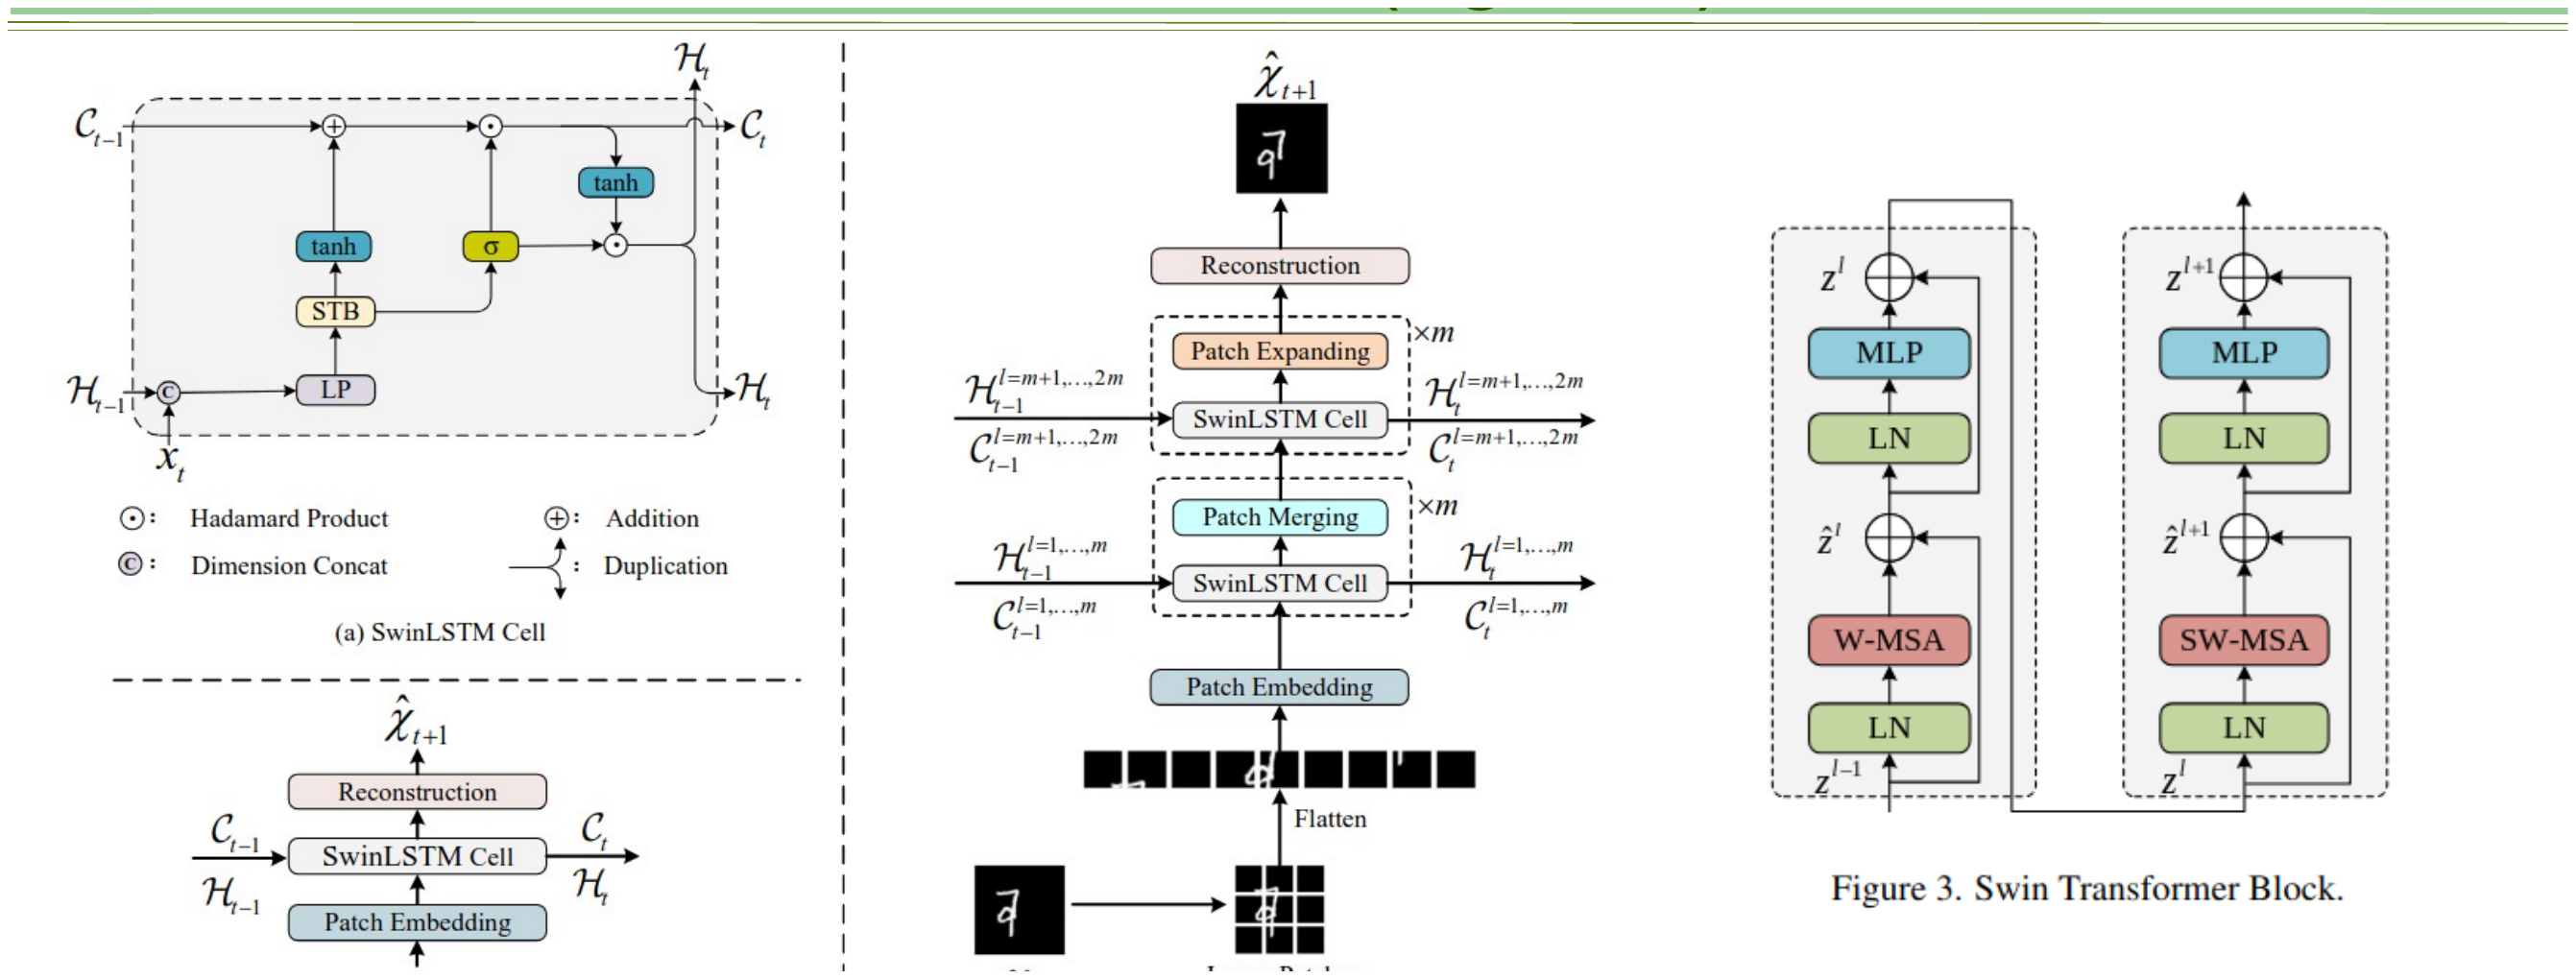
\includegraphics[width=\textwidth]{swinlstm}

    \vfill
    {\footnotesize
    Source: \url{https://github.com/SongTang-x/SwinLSTM}\\
    Being ported to \url{https://github.com/chengtan9907/OpenSTL} \hfill (Tang et al. 2023)}
\end{frame}

\begin{frame}{Future? Structured state space sequence models (SSM)}
    \begin{itemize}
        \item Linear or near-linear scaling in sequence length {\tiny (transformer grows quadratically)}
        \item Remove the nonlinearity in RNNs {\tiny (remember LSTM gates?)}
        \item Mamba: Linear-Time Sequence Modeling with Selective State Spaces (Gu et al. 2024) \url{https://github.com/state-spaces/mamba}
        \begin{itemize}
            \item Selection Mechanism
            \begin{itemize}
                \item Select data in an input-dependent manner
                \item SSM parameters based on the input
            \end{itemize}
        \end{itemize}
    \end{itemize}

    \begin{columns}[t]
        \column{0.45\textwidth}
        \centering
        {\footnotesize Linear recurrence computation}
        \begin{align*}
            h_t &= \overline{A} h_{t-1} + \overline{B} x_t \\
            y_t &= C h_t
        \end{align*}

        \column{0.5\textwidth}
        \centering
        {\footnotesize Global convolution computation}
        \begin{align*}
            \overline{K} &= (C\overline{B}, C\overline{AB}, \dots, C\overline{A}^k\overline{B}, \dots) \\
            y &= x * \overline{K}
        \end{align*}
    \end{columns}
\end{frame}

\begin{frame}{Future? Structured state space sequence models (SSM)}
    \begin{itemize}
        \item Video Mamba (Li et al. 2024):
        \begin{itemize}
            \item \url{https://github.com/OpenGVLab/VideoMamba}
            \item Designed for video classification, so we should have a forecast architecture soon.
        \end{itemize}
    \end{itemize}

    \centering
    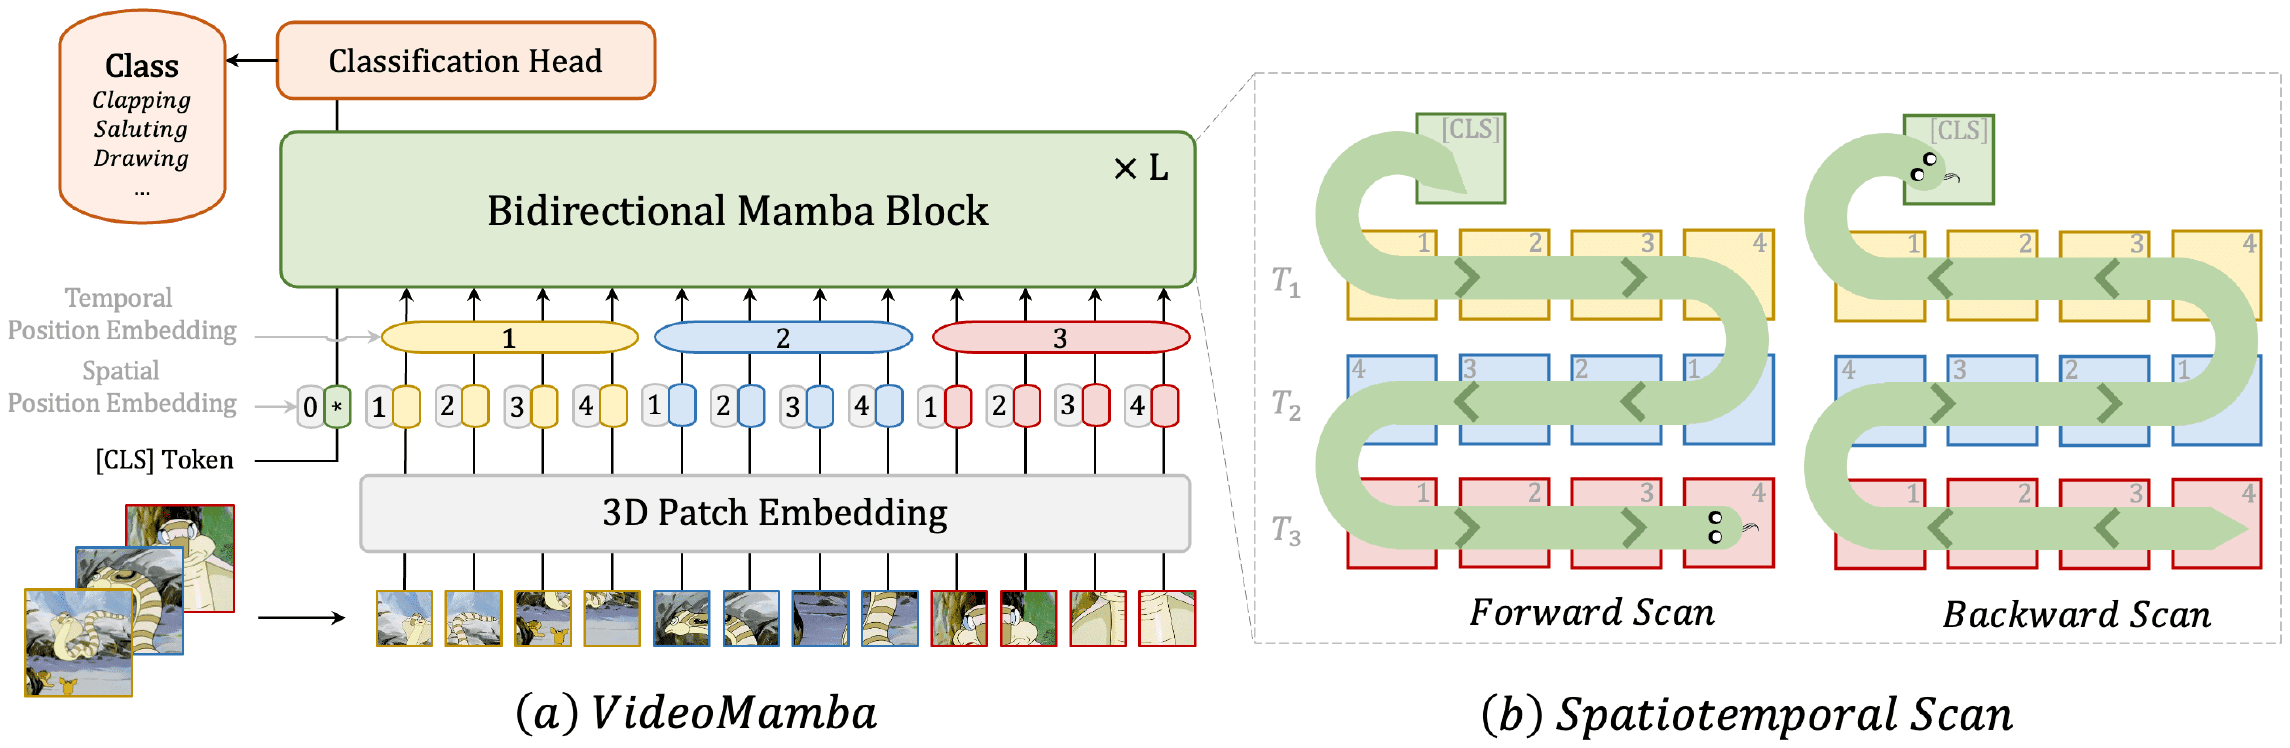
\includegraphics[width=0.9\textwidth]{videomamba}
\end{frame}

% ============================================================
\section{Hands on}
% ============================================================

\begin{frame}{OpenSTL (Pytorch+lightning)}
    \begin{columns}[c]
        \column{0.65\textwidth}
        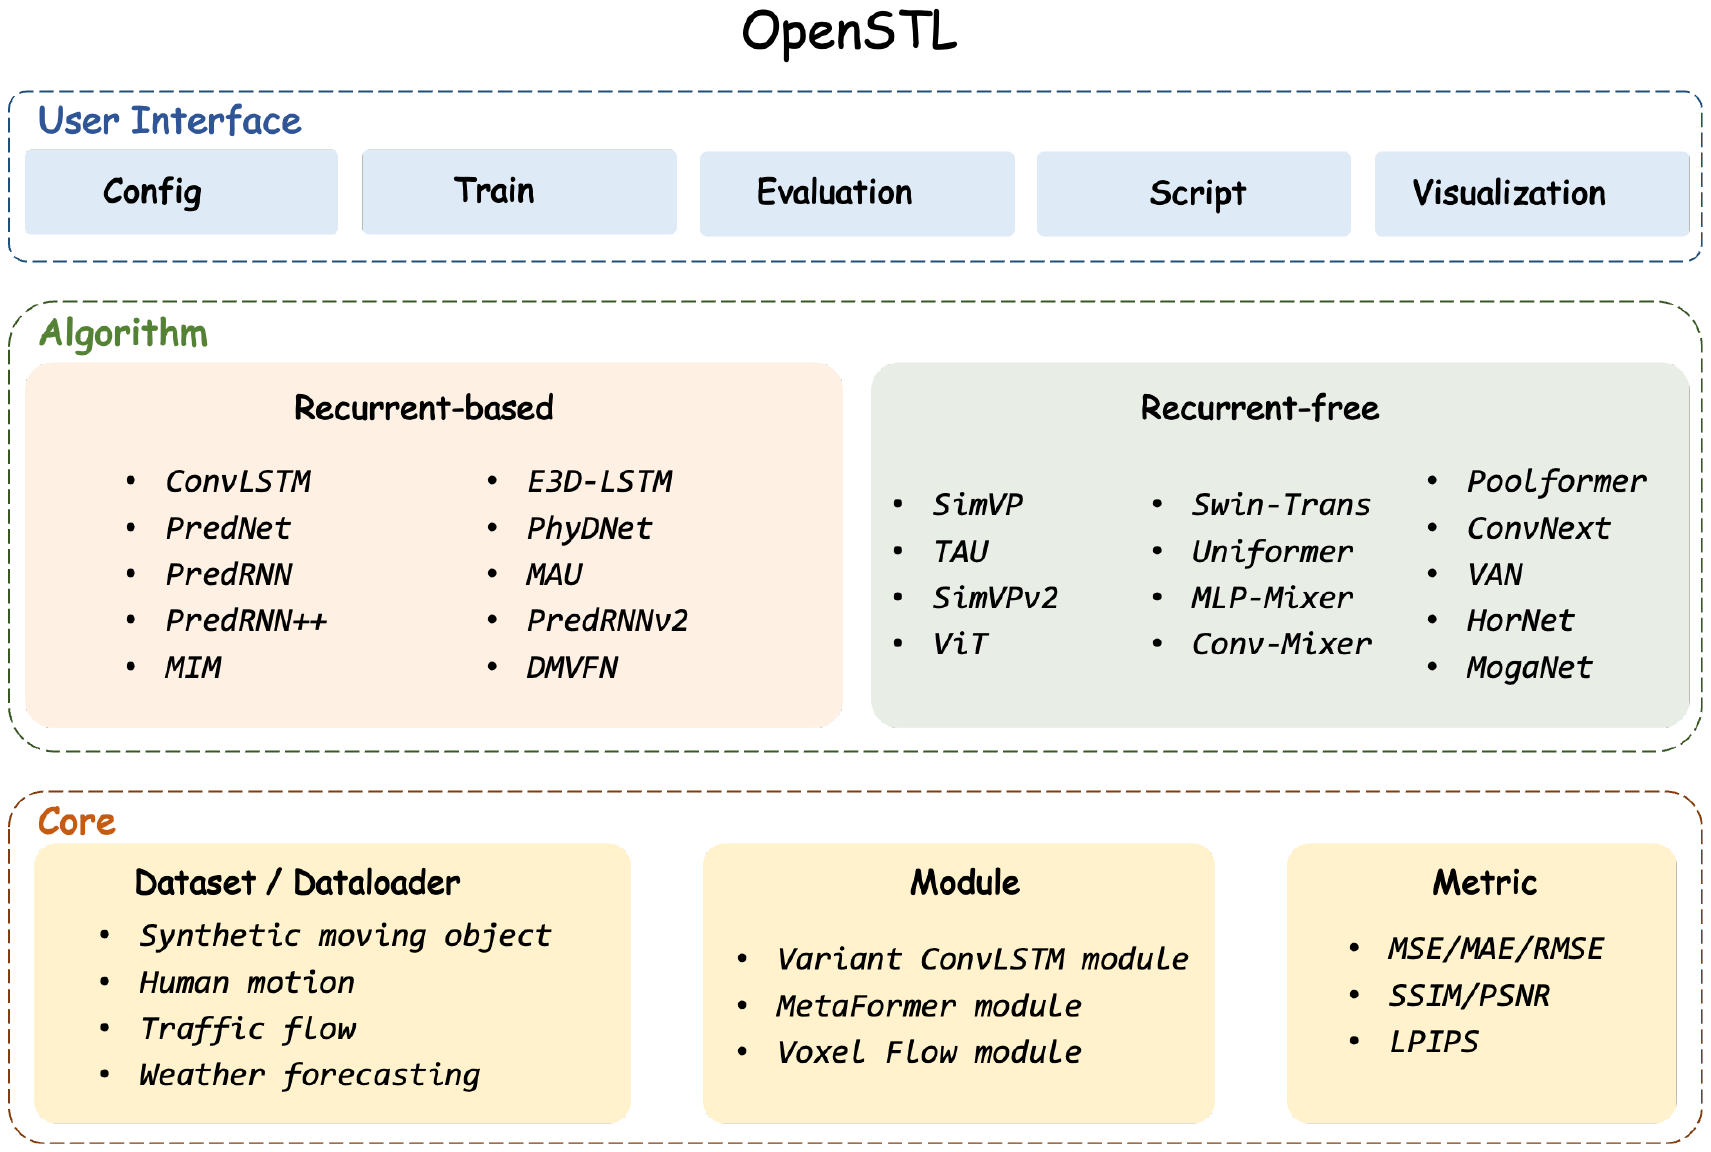
\includegraphics[width=\columnwidth]{openstl}

        \column{0.33\textwidth}
        \small
        \textbf{Possibilities}
        \begin{itemize}
            \item Create your dataloader and train a model.
            \item Use the models in your project.
            \item Create new models.
        \end{itemize}

        \textbf{What's the difference?}
        \begin{itemize}
            \item Learning capacity
            \item Memory
            \item Forecast procedure
            \item Training speed
            \item Prediction speed
        \end{itemize}
    \end{columns}

    \hfill{\tiny (Tan et al. 2023)}
\end{frame}

\begin{frame}{OpenSTL benchmark datasets (results)}
    \centering
    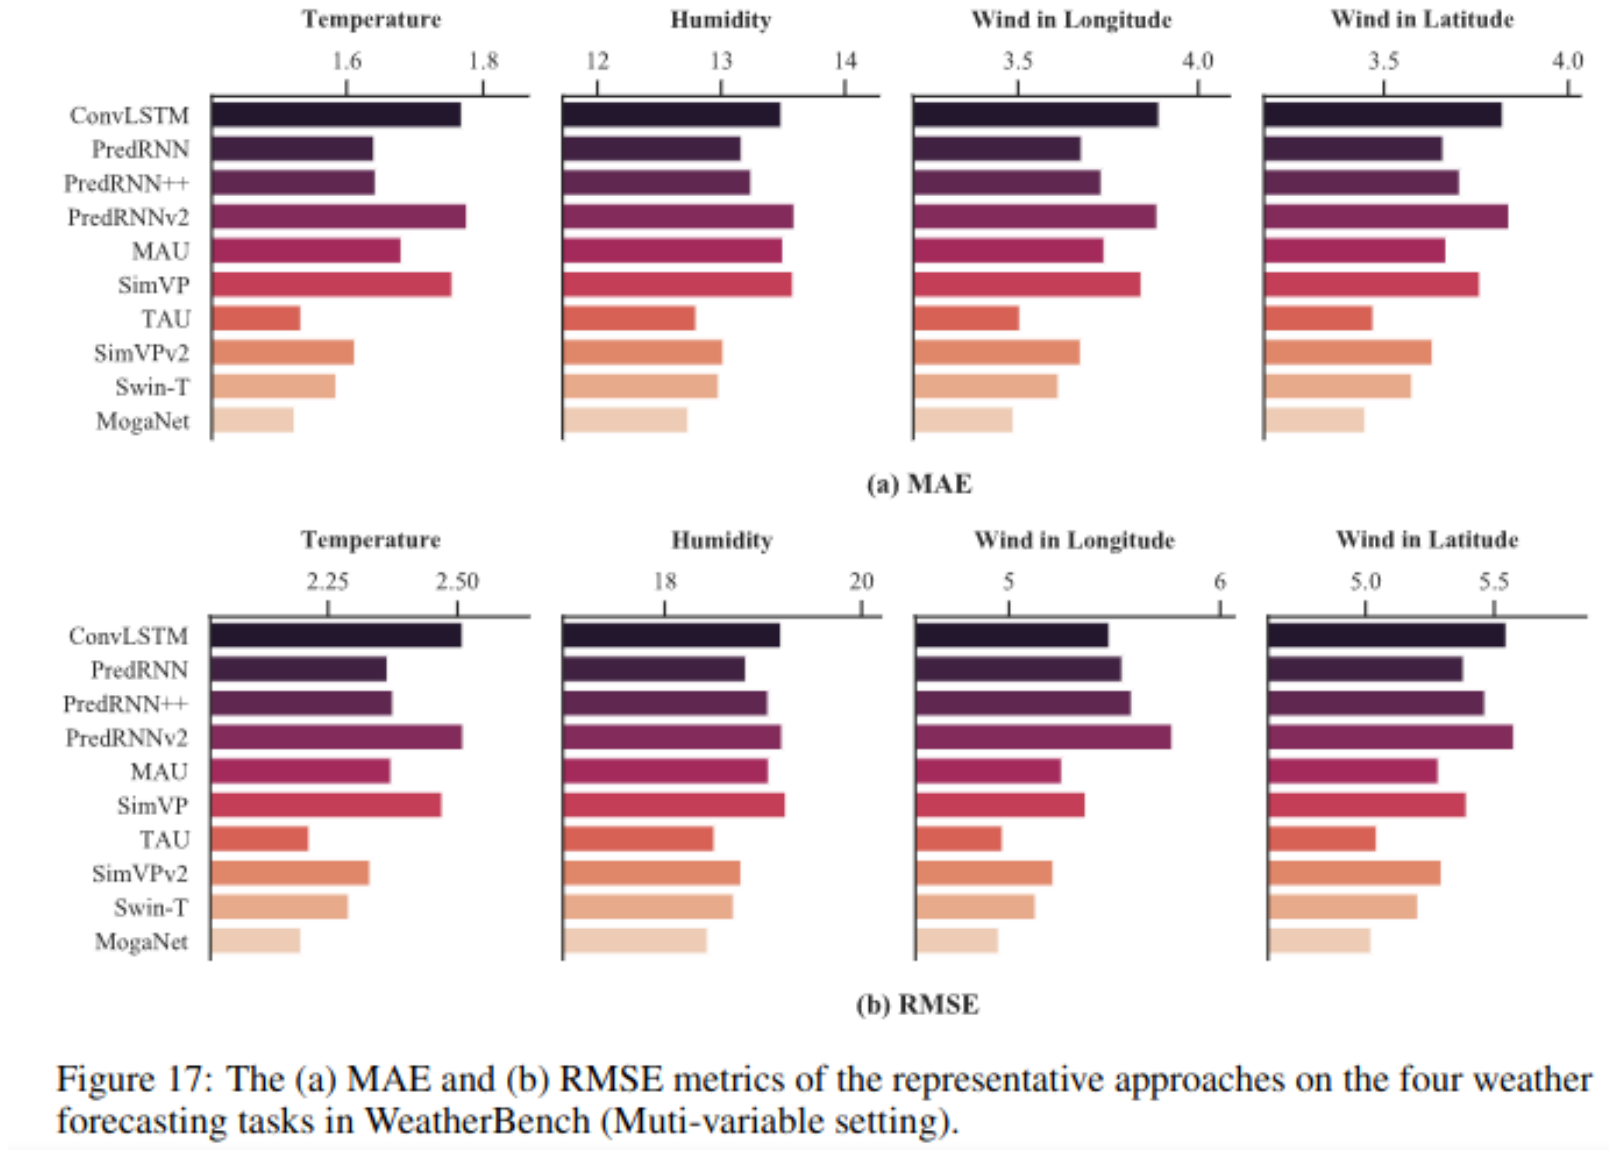
\includegraphics[height=0.8\textheight]{openstl_benchmark}

    \hfill{\tiny (Tan et al. 2023)}
\end{frame}

\begin{frame}{Google Colab code}
    \small
    \begin{itemize}
        \item \textbf{OpenSTL in Global Ionosphere Maps prediction (hands on)}
        \begin{itemize}
            \item \url{https://github.com/mauriciodev/tec_forecast/blob/main/examples/OpenSTL_GIM.ipynb}
        \end{itemize}
        \item OpenSTL custom dataloader tutorial
        \begin{itemize}
            \item \url{https://github.com/chengtan9907/OpenSTL}
            \item \url{https://colab.research.google.com/drive/19uShc-1uCcySrjrRP3peXf2RUNVzCjHh?usp=sharing}
        \end{itemize}
        \item GIM Forecast with PyTorch {\tiny (Paulo et al, 2023)}
        \begin{itemize}
            \item \url{https://github.com/mauriciodev/tec_forecast/blob/main/extra/tec_forecast_torch.ipynb}
        \end{itemize}
        \item GIM Forecast with Tensorflow/Keras {\tiny (Paulo et al, 2023)}
        \begin{itemize}
            \item \url{https://github.com/mauriciodev/tec_forecast/blob/main/examples/tec_forecast_tf2_lab.ipynb}
        \end{itemize}
    \end{itemize}
\end{frame}

% ============================================================
\section{Other topics}
% ============================================================

\begin{frame}{Loss functions and evaluation metrics}
    \begin{columns}[t]
        \column{0.58\textwidth}
        \textbf{Numerical prediction (Regression)}
        \footnotesize
        \begin{align*}
            MAE &= \frac{\sum_{i=1}^{n} |y_i - \hat{y}_i|}{n} \\
            RMSE &= \sqrt{\frac{\sum_{i=1}^{n} (y_i - \hat{y}_i)^2}{n}} \\
            Huber &= \frac{\sum_{i=1}^{n} L_{huber}(y, \hat{y})}{n}
        \end{align*}
        where $L_{huber}(y,\hat{y}) =
        \begin{cases}
            \frac{1}{2}(y - \hat{y})^2 & \text{for } |y - \hat{y}| < \delta \\
            \delta \left(|y - \hat{y}| - \frac{1}{2}\delta\right) & \text{otherwise}
        \end{cases}$
        \[
        R^2 = 1 - \frac{\sum_{i=1}^{n} (y_i - \hat{y}_i)^2}{\sum_{i=1}^{n} (y_i - \bar{y})^2}
        \]

        \column{0.4\textwidth}
        \textbf{Categorical prediction}
        \begin{itemize}
            \item Categorical cross entropy loss
            \item Focal loss
            \item Precision, recall, F-score
            \item Intersection over union (IOU)
        \end{itemize}

        \vfill
        \scriptsize
        $n$: Number of samples in a batch\\
        $y$: Values from the training sample;\\
        $\hat{y}$: Values predicted with the network.
    \end{columns}
\end{frame}

\begin{frame}{Exploring the results}
    \begin{columns}[c]
        \column{0.5\textwidth}
        \centering
        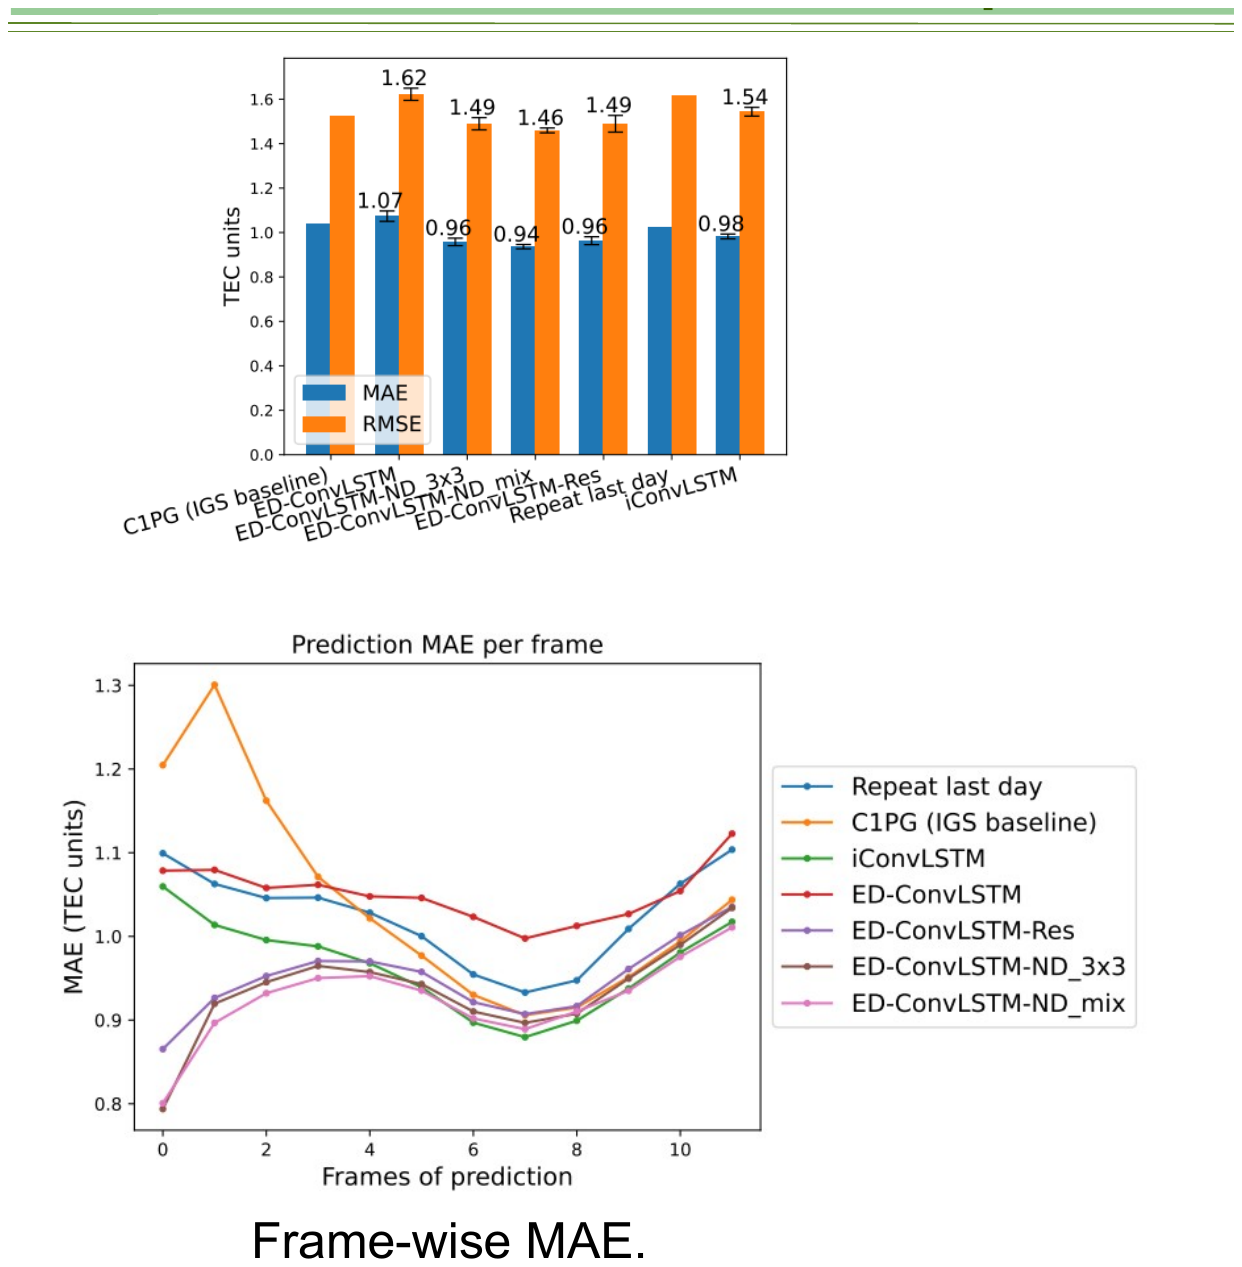
\includegraphics[height=0.78\textheight]{results_mae}

        \column{0.48\textwidth}
        \centering
        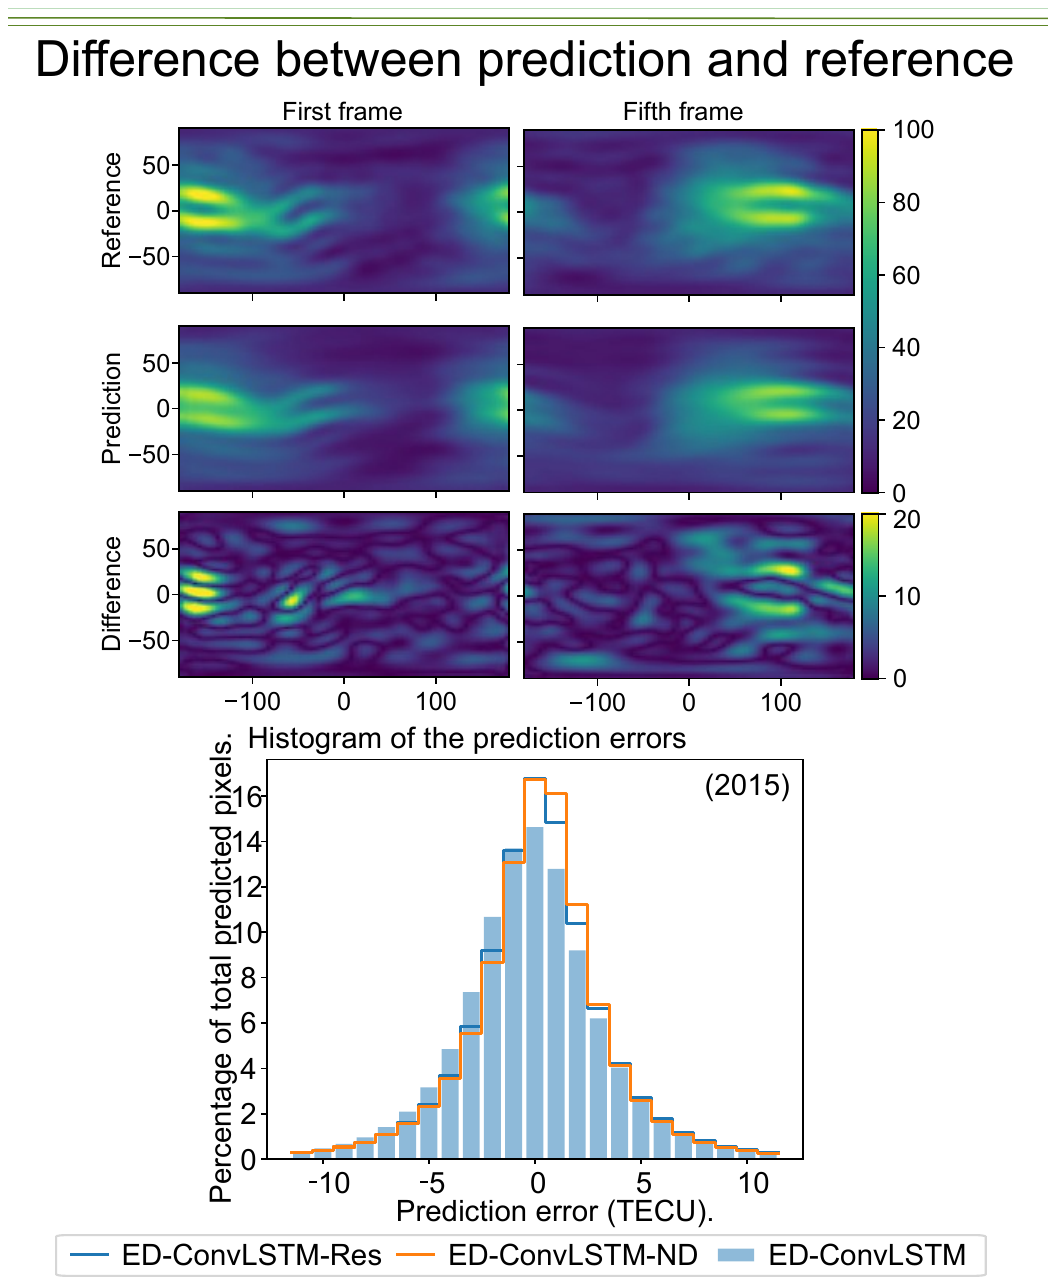
\includegraphics[height=0.8\textheight]{results_maps}
    \end{columns}
\end{frame}

\begin{frame}{Data set construction: What do we measure?}
    \centering
    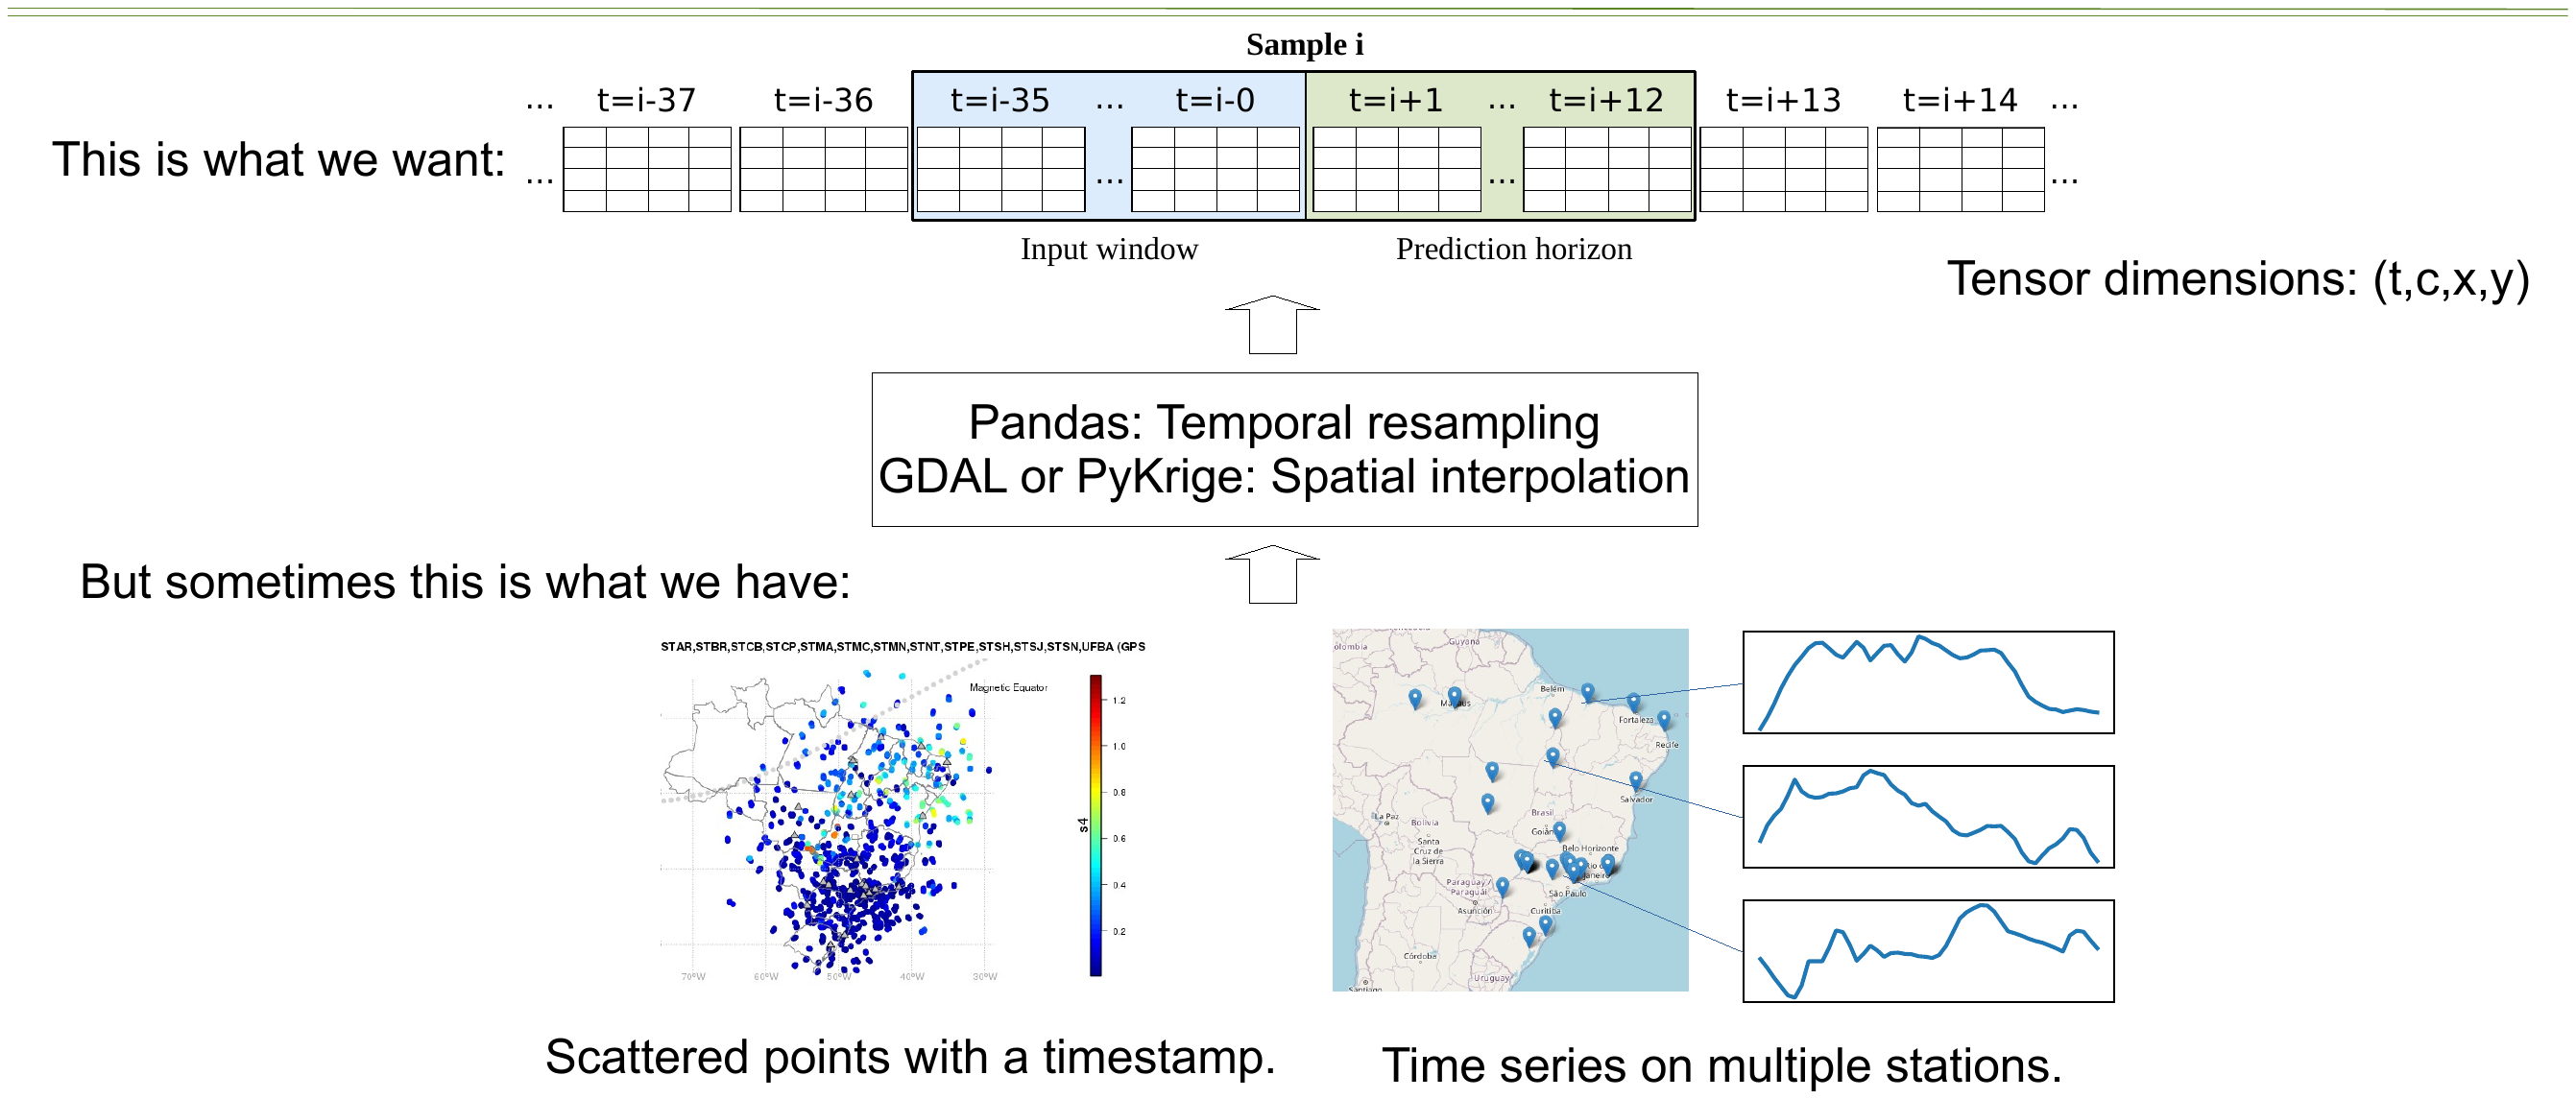
\includegraphics[width=\textwidth]{what_we_measure}

    \hfill Among others (1D? Graphs?)
\end{frame}

\begin{frame}{Convolutional layers dimensions}
    \begin{columns}[c]
        \column{0.72\textwidth}
        \begin{itemize}
            \item Popular pooling options:
            \begin{itemize}
                \item Max
                \item Average
            \end{itemize}
            \item Spatial pooling
            \begin{itemize}
                \item $(t, x, y, c) \rightarrow (t, x/2, y/2, c)$
            \end{itemize}
            \item Temporal pooling
            \begin{itemize}
                \item $(t, x, y, c) \rightarrow (t/2, x, y, c)$
            \end{itemize}
            \item Spatiotemporal pooling (uncommon)
            \begin{itemize}
                \item $(t, x, y, c) \rightarrow (t/2, x/2, y/2, c)$
            \end{itemize}
            \item \textbf{Convolution with stride can change resolution too.}
            \item Spatial and temporal resolution changes must make sense for the event.
        \end{itemize}

        \column{0.26\textwidth}
        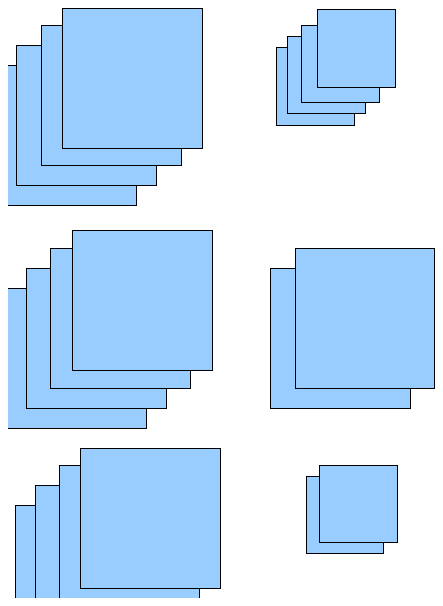
\includegraphics[width=\columnwidth]{pooling}
    \end{columns}
\end{frame}

\begin{frame}{Convolutional layers dimensions}
    \begin{columns}[c]
        \column{0.38\textwidth}
        \small
        \begin{itemize}
            \item \textbf{Dilated convolution}
            \begin{itemize}
                \item Spatial
                \item Temporal
                \item Spatiotemporal (uncommon)
            \end{itemize}
            \item \textbf{Deformable}
        \end{itemize}
        
        \column{0.6\textwidth}
        \centering
        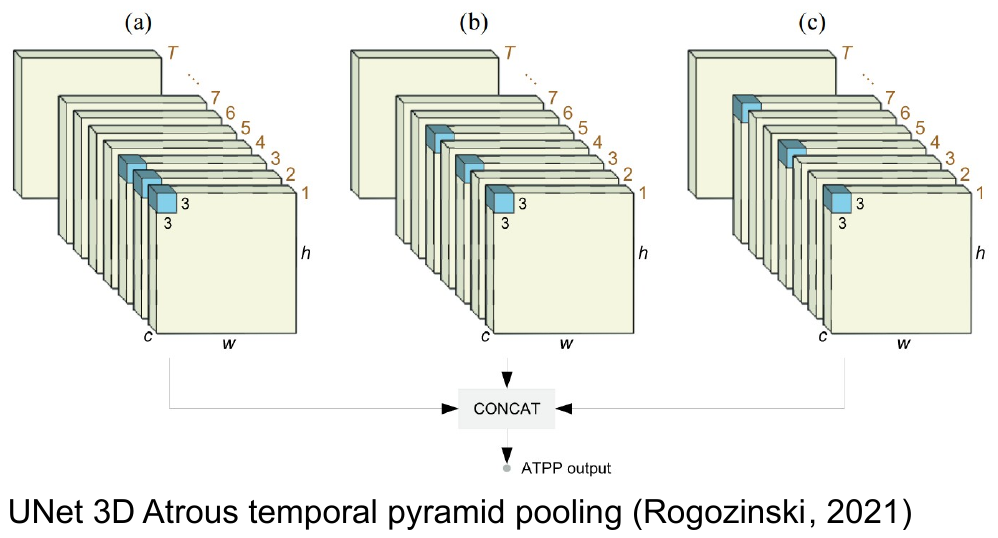
\includegraphics[height=0.3\textheight]{atrous_unet3d}
    \end{columns}
    
    \vfill
    \begin{columns}[b]
        \column{0.3\textwidth}
        \centering
        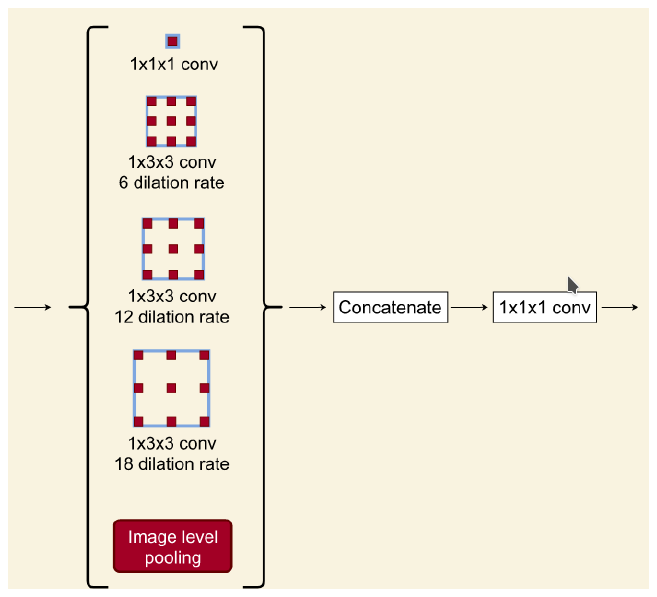
\includegraphics[height=0.3\textheight]{atrous_broadunet}
        
        {\tiny Broad-UNet Atrous spatial pyramid pooling (Fernández, 2021)}
        
        \column{0.38\textwidth}
        \centering
        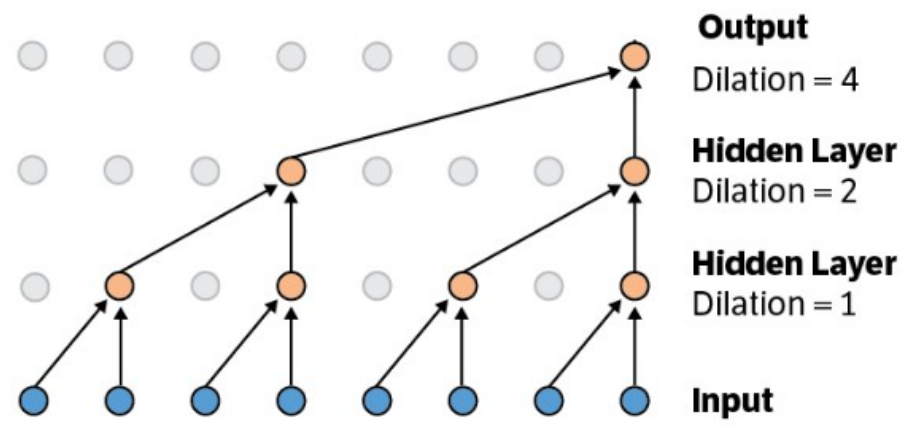
\includegraphics[height=0.22\textheight]{wavenet}
        
        {\tiny Wavenet's sequence of time dilated convolutions (Borovykh, 2018)}
        
        \column{0.28\textwidth}
        \centering
        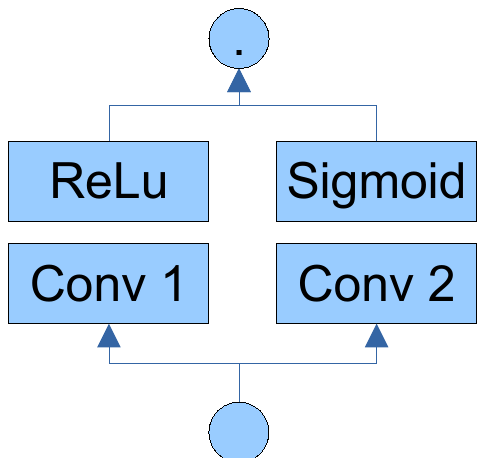
\includegraphics[height=0.22\textheight]{sigmoid_gate}
        
        {\tiny Sigmoid gates control the output of a block.}
    \end{columns}
\end{frame}

% ============================================================
\section{Referências}
% ============================================================

\begin{frame}[allowframebreaks]{Referências}
    \tiny
    \begin{itemize}
        \item[] Arnab A, Dehghani M, Heigold G, Sun C, Lucic M, Schmid C (2021) ViViT: A Video Vision Transformer. In: 2021 IEEE/CVF International Conference on Computer Vision (ICCV). IEEE, Montreal, QC, Canada, pp 6816--6826
        \item[] Beck M, Pöppel K, Spanring M, Auer A, Prudnikova O, Kopp M, Klambauer G, Brandstetter J, Hochreiter S (2024) xLSTM: Extended Long Short-Term Memory
        \item[] Borovykh A, Bohte S, Oosterlee CW (2018) Conditional Time Series Forecasting with Convolutional Neural Networks. arXiv:170304691 [stat]
        \item[] Dosovitskiy A, Beyer L, Kolesnikov A, Weissenborn D, Zhai X, Unterthiner T, Dehghani M, Minderer M, Heigold G, Gelly S, Uszkoreit J, Houlsby N (2021) An Image is Worth 16x16 Words: Transformers for Image Recognition at Scale
        \item[] Fernández JG, Mehrkanoon S (2021) Broad-UNet: Multi-scale feature learning for nowcasting tasks. Neural Networks 144:419--427. \url{https://doi.org/10.1016/j.neunet.2021.08.036}
        \item[] Gao Z, Shi X, Wang H, Zhu Y, Wang B, Li M, Yeung D-Y (2022) Earthformer: Exploring Space-Time Transformers for Earth System Forecasting
        \item[] Li K, Li X, Wang Y, He Y, Wang Y, Wang L, Qiao Y (2024) VideoMamba: State Space Model for Efficient Video Understanding
        \item[] Li S, Wang Z, Liu Z, Tan C, Lin H, Wu D, Chen Z, Zheng J, Li SZ (2023) Efficient Multi-order Gated Aggregation Network
        \item[] Paulo MCM de, Marques HA, Feitosa RQ, Ferreira MP (2023) New encoder--decoder convolutional LSTM neural network architectures for next-day global ionosphere maps forecast. GPS Solut 27(2):95. \url{https://doi.org/10.1007/s10291-023-01442-4}
        \item[] Paulo MCM de, Marques HA, Ferreira MP, Feitosa RQ (2022) Redes neurais ConvLSTM CD aplicadas à previsão de mapas globais de ionosfera. In: Informações geoespaciais para o monitoramento do sistema terra visando o desenvolvimento sustentável. Curitiba, Brasil
        \item[] Rogozinski M, Martinez JAC, Feitosa RQ (2021) 3D convolution for multidate crop recognition from multitemporal image sequences. International Journal of Remote Sensing 0(0):1--22. \url{https://doi.org/10.1080/01431161.2021.1976876}
        \item[] Tan C, Gao Z, Li SZ, Li S (2022) SimVP: Towards Simple yet Powerful Spatiotemporal Predictive Learning
        \item[] Tan C, Li S, Gao Z, Guan W, Wang Z, Liu Z, Wu L, Li SZ (2023) OpenSTL: A Comprehensive Benchmark of Spatio-Temporal Predictive Learning
        \item[] Tang S, Li C, Zhang P, Tang R (2023) SwinLSTM: Improving Spatiotemporal Prediction Accuracy using Swin Transformer and LSTM
        \item[] Vaswani A, Shazeer N, Parmar N, Uszkoreit J, Jones L, Gomez AN, Kaiser L, Polosukhin I (2017) Attention Is All You Need
    \end{itemize}
\end{frame}

\end{document}
